\documentclass[12pt]{article}

\pdfminorversion=4

\usepackage[utf8]{inputenc} %unicode support

\usepackage{amsmath}
\usepackage{amssymb}
%\usepackage{pdfpages}
\usepackage{gensymb}
\usepackage{graphicx}
\usepackage{epstopdf}
\usepackage{color}
\usepackage[margin=1in]{geometry}
\usepackage{times,mathptmx}

% Bold the 'Figure #' in the caption and separate it with a period
% Captions will be left justified
\usepackage[labelfont=bf,labelsep=period,justification=raggedright]{caption}

% Use the ACS provided bibtex style
%\bibliographystyle{plain}
\bibliographystyle{acs}
\usepackage{cite}

% Remove brackets from numbering in List of References
\makeatletter
\renewcommand{\@biblabel}[1]{\quad#1.}
\makeatother


% definition of \customlabel, which is used to label supplementary figures and tables
\makeatletter
\newcommand{\customlabel}[2]{%
\protected@write \@auxout {}{\string \newlabel {#1}{{#2}{}}}}
\makeatother


\begin{document}


\title{Large-scale analysis of post-translational modifications in \emph{E. coli} under glucose-limiting conditions over 2 weeks}

\author{Viswanadham Sridhara$^1$, Colin Brown$^{2}$, Daniel R. Boutz$^{2,3}$, Maria Person$^{4}$,\\
Jeffrey E. Barrick$^{1,2,3,5}$, Edward M. Marcotte$^{1,2,3,5}$, and Claus O. Wilke$^{1,2,3,5,6}$}
\maketitle

\noindent
$^1$Center for Computational Biology and Bioinformatics, The University of Texas at Austin, Austin, TX, USA\\
$^2$Institute for Cellular and Molecular Biology, The University of Texas at Austin, Austin, TX, USA\\
$^3$College of Pharmacy, The University of Texas at Austin, Austin, TX, USA\\
$^4$Center for Systems and Synthetic Biology, The University of Texas at Austin, Austin, TX, USA\\
$^5$Department of Molecular Biosciences, The University of Texas at Austin, Austin, TX, USA\\
$^6$Department of Integrative Biology, The University of Texas at Austin, Austin, TX, USA\\


\begin{abstract}
How do the post-translational modifications change over time during microbial growth under nutrient limiting conditions? We sought to answer this question using \emph{E. coli} grown under glucose starvation conditions. We generated mass-spectrometry based proteomics data at 9 different time points ranging from exponential to long stationary phases i.e., 2 weeks. We then ran MODa on this data for an unrestricted search of PTMs. There were several interesting observations in this MODa analysis. First, we show that the amount of modified protein seems to be constant, occuring approx. 30\%, at all the 9 time points. Second, we show that acetylations, carboxylations and phosphorylations increase, while nitrosylations seem to be constant from exponential to stationary phases.Third, we show that sulfoxide reductases fix MetSO to Met during stationary phase, protecting \emph{E. coli} from oxidative damage. Finally, we found some novel post-translational modifications in this data, a frequent one being phosphogluconylation on serine in R6 ribosomal protein.
\end{abstract}

% keywords: post-translational modifications

\section{Introduction}

Mass-spectrometry based proteomics offers a uniquie way to characterize different post-translational modifications [PTMs] associated with proteins. PTMs are key in determining protein function, localization and regulation. Hundreds of PTMs are known \emph{in vivo}, however most of the current studies focus on identifying few PTMs from mass-spec data. This is both because of computational limitations as well as the inefficiency of enrichment techniques to characterize or identify all PTMs. In the last decade, however there has been lot of effort to improve search algorithms to increase the coverage of PTMs i.e., using unrestricted naive based search instead of traditional search, where a guessed list of only handful PTMs is provided beforehand.

In this study, we are interested in identifying/characterizing different PTMs in \emph{E. coli} grown under glucose limiting conditions. \emph{E. coli} grown under these nutrient limiting conditions generally behave differently at different phases of their growth i.e., during exponential and stationary phases. During the stationary phase, stress response proteins act because of the conditions casued by limiting nutrients, change in pH value, accumulation of toxic substances in the flasks etc. In an earlier study under similar conditions, the number of phosphorylation sites as well as their occupancy levels seem to increase during stationary phase as a response to stress. In the same study, protein abundance of SspA seemed to be constant, while the phosphorylation of the same protein increased suggesting PTM level quantitation as key compared to protein quantitation. In another study by the same group, the oxidative stress has been shown to be compensated by the E. coli machinery at the later stages of growth i.e., stationary phase compared to the early exponential phase. This itself suggests that PTM level stoichiometry is necessary to understand the response of organisms to environmental and other disturbances.

Other studies on PTMs focussed on multiple PTMs, but they looked at only one "snapshot" of interest. This information is insufficient to explain the significance or the function associated by PTMs. Few sites have been previously shown to be modified by different PTMs depending on the circumstances. So, analyzing multiple PTMs in tandem is necessary to understand behavior of microbes under different conditions. Here, we argue that we need a comprehensive analysis of PTMs at different time points to understand the PTM level response. 

Our earlier work using the protein, mRNA, lipid and metabolite level information at different phases in growth suggested the significance of such comprehensive analysis. However, we did not focus our earlier work at PTM level, but instead analyzed the protein abundances. Here, we did an unrestricted search to identify most of the PTMs and at 9 different time points during the exponential and long-stationary phases lasting upto 2 weeks.

\section{Results}

\subsection{Running MODa on \emph{E. coli} proteome}
Post-translational modifications, in most cases, determine the specific function of the protein. Identifying all the PTMs associated with proteins is limited by both experimental enrichment techniques for PTMs as well as computational limitations. The current dataset is not enriched for any PTMs, however we are interested in identification of different kinds of PTMs, instead of focussing on single PTMs, such as generally done in phosphoproteomics studies, glycosylation studies or acetylation studies. Here, we used a search algorithm MODa, which uses an unrestricted approach to find the post-translational modifications in the data. Our goal is not only to identify the PTMs present in the sample, but also understand the time evolution of these PTMs from exponential phase (3,4,5,6 hours of growth) to long-stationary phases (8,24,48, 168 and 336 hours). OD600 at these 9 time points is given in supplementary information of this article (see Suppl Figure S1). For this analysis, we ran MODa using the parameteres specified in detail in methods section below. In brief, MODa finds multiple short sequence tags and then uses a dynamic programming technique to identify the peptide hits. Use of multiple tags reduces the database size. 

%The mass-spectrometry data gathered at the 9 time points is then searched for PTMs using MODa, a naive based spectral alignment search algorithm, for peptide identifications. At each of these 9 time points, we gathered data for 3 biological replicates. Unlike most of the other peptide identification search algorithms, MODa requires range of mass for PTM identification. So, for our analysis we used a range of -200 to 200 Da which is typical to this search engine. MODa is a multi-blind algorithm i.e., there is no restriction on the  number of PTMs identified on a single peptide. However previous studies have shown better sensitivity of the algorithm with the use of 1 mod per peptide. We used 1 mod per peptide for most of the analysis, however we compared our results with using 2 mods per peptide too.

We asked the following questions using our MODa output on peptide identifications:
(a) How much of the proteome is modified? (b) How do these modifications change over time and is there any biological relevance associated with this temporal change? (c) Can we find any novel modifications? 

%(d) Can we explain the pattern of the PTMs over time using other diverse kinds of data such as RNA-seq? In this project, we also collected mRNA via RNA-seq, lipid profiles and metabolic fluxes using mass-spec methods. We went back and compared our proteomics data with these other kinds of data for further validation, wherever necessary.

\subsection{Modified \emph{E. coli} proteome}
First, we are interested in understanding how much of the proteome is modified at each of the 9 time points i.e., from exponential to long-stationary phases? For this, we calculated the percentage of the total number of modified peptides in the peptide spectral matches (PSMs) list. We used 1 standard error to plot the variation within 3 biological replicates.

Figure~\ref{fig:ModifiedPTM} shows the total percent of the peptide-spectral matches on the y-axis and the time on the x-axis. As it can be seen, the number of modified spectra is ~30\% at all the time points. The ~30\% of protein getting modified is in agreement with some of the previous studies (Cite papers which show the same numbers). However previous studies did not look at the temporal change or look at the change in each of the specific PTMs of interest. Our analysis, as shown below, points to specific PTMS that increase/decrease or remain constant over time.

%However note that a modification could be a mutation or a post-translational modification.
\subsection{Mapping mass-shifts to post-translational modifications}
To look at the specific PTMs, we need to convert the mass-shifts outputted by MODa to the PTMs of interest i.e., +16Da is most likely the oxidation. For this conversion, we used UNIMOD database that lists the PTMs along with their masses in daltons. We looked only at handful of well known PTMs. In this study, we limited our analysis to few post-translational modifications and did not investigate mutations, although this is a possibility with MODa output.
%MODa outputs not only the mass-shifts, but also the amino-acids on which this mass-shift occurs. We focussed not only on the most common PTM-amino acid combinations, but also on the PTMs irrespective of the amino acid. 
%To understand what kinds of PTMs (or mutations) are present in the sample, we plotted the frequency of the mass-shifts. MODa program outputs the frequency of mass-shifts in intervals of 1Da, along with the amino acid on which this mass-shift occurs.
%Along with the amino acids, it also calculates the N-term and C-term mass-shifts. 
Figure~\ref{fig:PTMinDalton} shows the mass-shift frequency matrix. (A) shows the distribution at 3 hours and (B) at 24 hours. We did not plot the error bars as this makes the figure a bit clumsy, with error bars appearing at each bin. These are the means of the 3 biological replicates. The error bars indicate 1 standard error. It is clear that +1 Da peak is the most frequent one. However this +1 Da modification seems to be 13C peak-picking as it seems to be randomly occuring on all the amino acids, as shown in the profile (Suppl Figure S5). At both 3 and 24 hours, next frequent modification seems to be the bin at +16Da. 16Da indicates oxidation and cysteine and methionine are the 2 most frequent amino acids that are oxidized. However, the sample is treated in a way to cap cysteines and hence we dont expect to see Cys oxidized. A look at profile (Suppl Figure S6) shows majority of oxidations on methionine which is expected. Similarly, we mapped other frequent and known mass-shifts and looked at their temporal analysis. In particular, we looked at  acetylation, oxidation, phosphorylation, carboxylation and nitrosylation in depth.

\subsection{N-term protein acetylations are frequent in \emph{E. coli}}
 
Acetylation in \emph{E. coli} has been studied well in the past \cite{Charbautetal2002} \cite{Gordiyenkoetal2008}. Acetylation occurs in 2 forms i.e., N-{alpha} acetylation and N-{sigma} acetylation. It is known that acetylation occurs co-translationally on n-term (N-{alpha}) and is not reversible, while post-translationally it occurs as a reversible modification, mostly on lysine  (cite this paper) \emph{The diversity of lysine-acetylated proteins in Escherichia coli.}. In the current work, we focus on n-terminal acetylation. It has been known that almost 2/3rds of the proteins are substrates for n-terminal methionine excision. Following this methionine excision, n-terminal processing, especially n-terminal acetylation \cite{Driessenetal1985} has been shown in the past to be one of the most frequently occuring PTMs. Previous data suggests that this modification is more frequent in eukaryotes than bacteria. However our results indicate that there are quite a few n-term protein acetylations identified. We summarize our results below. 

N-terminal acetyltransferases are responsible for the n-terminal acetylation \cite{Starheimetal2012}.  Irrespective of the type of acetylation, since MODa allowed us to look at the global acetylation level i.e., all possible shifts of 42Da, we plotted the acetylation frequencies at different time points as a function of time (see Figure~\ref{fig:Acet}). The total number of acetylations seem to go up from exponential to stationary phases. In our analysis, most of the acetylations seem to be protein n-term acetylations. Either this acetylation occurs on the 1st methionine amino acid or it happens on the 2nd amino acid after the excision of the 1st methionine. Figure~\ref{fig:Acet} also shows the total n-term acetylations and the total serine acetylations. Later, we show that the serine acetylations seem to happen >99\% of the times at n-term.

E. coli grown on glucose have shown to accumulate acetate (Cite proper references). Our results might suggest the same given the increase in the number of acetylated proteins from exponential to stationary phases. Table 1 shows the acetylated proteins found under these 2 different phases under E. coli growth under glucose limiting conditions.

{Colin Brown's analysis could go here}

%(May be add a figure on n-terminal processing percentage of acetylation either in supplementary or in main paper?) Also add a table that has a list of acetylated proteins.

Out of 3919 total acetylations at all 9 time points combined, 3373 (86\%) of them seem to occur at n-term of the protein. A look-up of the amino acid position for n-term acetylations on ID'ed peptides showed that these were the 2nd amino acid in most (quote?) of the cases. {May be add about the signal peptides here}. Also, most of the acetylations seem to occur on serine (2358 out of 3919). Among n-term protein acetylations, 2350 (70\%) happened on serine, 483 (14.3\%) happened on alanine and 260 (7.7\%) were on threonine. These were the top 3 frequent n-term acetylations. A literature search also showed us the same frequently occuring n-term acetylated amino acids in E. coli {cite}.


\subsection{\emph{E. coli} Phosphorylations, carboxylations, nitrosylations and other PTMs}

Next we analyzed other PTMs that were previously shown to be key in E. coli. In particular, we looked at phosphorylation, carboxylation, nitrosylation and oxidation. As mentioned earlier, a key point to note in this analysis is that there is no enrichment done for any of these PTMs, hence the coverage will be smaller than expected. Typical studies that identify phosphopeptides are generally enriched for phosphorylations using enrichment techniques such as IMAC, TiO2 etc. However as we mentioned early, our goal here is to identify different kinds of PTMs in this proteomics data and look at how they change over time. Figure~\ref{fig:Phos} shows the phosphorylations at different points of the growth curve. Here, we counted the phosphorylations on Serine, Threonine and Tyrosine only as they seem to be well known amino acids that get phosphorylated \cite{Maceketal2008}. There are 2 interesting observations seen in this curve. First, the number of phosphorylations seem to be small as expected, as these are not enriched for phosphorylations and moreover, the number of phosphorylations seem to be comparatively lower in E. coli. Second, and probably an interesting observation is that there is an increase of the number of phosphorylations from exponential to stationary phases. Such pattern is also previously shown in phosphoproteomic studies \cite{Soaresetal2013} probably pointing to a role of phosphorylation in later stages of the growth cycle.

Similarly we looked at the carboxylations (See Suppl Figure S2)and nitrosylations (See Suppl Figure S3), as they are shown in the past to be important in E. coli. Like, phosphorylations, carboxylations seem to increase during the later stages of the growth indicating a likely role of this PTM in late stationary phase. (There are studies linking cellular growth rate to carboxylases, may be related to what is shown here?) A previous study in S-nitrosylation in E.coli \cite{Sethetal2012}. We found succinylation modification frequently at different phases, all on the succinyl-transferase. This was previously characterized in a study where the authors were analyzing data for succinylation. Here we would like to point out that this large-scale study to analyze different PTMs without any enrichment was able to identify and characterize widely occuring PTMs generally identified in E. coli. 

An artifact caused by sample preparation and mass-spectrometry analysis is the adduct formation with Na and K. Here, we plotted the profiles of Na and K adducts (see Suppl Figure S4). Na and K adducts don't seem to form on H, K and R compared to other amino acids. These are amino acids that have side chains that are basic and carry a small positive charge at physiological pH. This explains why the adducts don't form with these amino acids. We give a general recommendation to include these adducts as variable modifications in the search engines to increase the sensitivity of the peptide identifications. Most of the software have an easy option to include these adducts and hence we recommend this giving a 3-4\% increase in identifications.

Glutamine conversion at n-term of the peptide to pyroglutamate is a well known PTM. This post-translational modification stabilizes the protein to avoid any further n-terminal processing. Suppl Figure 7 shows that this conversion seems to be more or less same at different phases of the growth.

\subsection{Oxidative damage and repair in \emph{E. coli}}
%\cite{Vogt1995}
%{Oxidation of methionyl residues in proteins: tools, targets, and reversal}
%
%\cite{Tete-Favieretal2000}
%{Crystal structure of the Escherichia coli peptide methionine sulphoxide reductase at 1.9 A resolution}
%   
%\cite{Tete-Favieretal2000b}
%{Crystallization and preliminary X-ray diffraction studies of the peptide methionine sulfoxide reductase from Escherichia coli}
%   
%\cite{ZhangWeissbach2008}
%{Origin and evolution of the protein-repairing enzymes methionine sulphoxide reductases}
%   
%This fixation of MsrA is helpful \cite{Abramsetal1981}
%{Enzymatic reduction of oxidized alpha-1-proteinase inhibitor restores biological activity}
%
%\cite{Davisetal2000}
%{HIV-2 protease is inactivated after oxidation at the dimer interface and activity can be partly restored with methionine sulphoxide reductase}
Next, we looked into oxidation of methionine. Oxidation generally occurs frequently on cysteine and methionine. However since cysteine is capped to avoid disulphide bond formation in these experiments, we expect +16Da shift to occur frequently on methionone. Other than cysteine and methionine, there are 8 other amino acids that have been shown to be oxidized although at a lower rate and less frequent. 

E. coli grown aerobically react with oxygen in the atmosphere producing reactive oxygen species such as H2O2 {CiteGonzalez-Flecha B, Demple B (1995) Metabolic sources of hydrogen peroxide in aerobically growing Escherichia coli. J Biol Chem 270: 13681–13687}. Targets for these ROS are generally proteins and lipids, that get oxidized. This oxidized state affects the protein structure and hence results in changes in its function leading to disturbances in the metabolism. Bacteria have genetic systems that responds to this oxidative stress through oxyR, SoxXY etc or through reductases that reduce protein to its original non-oxidized state. Here, we investigated the levels of oxidation at different phases of growth.

Figure~\ref{fig:Oxid} (A) shows the global oxidation levels occuring on all amino acids. The oxidations seem to go down from exponential to stationary to long stationary phases. Figure~\ref{fig:Oxid} (B) shows the oxidation occuring on methionine only. The pattern seems to be same as the global oxidation level i.e., goes down from exponential to stationary phases. This result seemed strange as we expected oxidative stress to increase under these glucose-starvation conditions in \emph{E. coli}. May be the bacterial genetic systems that respond to oxidative stress are acting to bring back the oxidation levels down. To validate this, we looked into literature to look into reduction systems that fix methionine sulfoxide back to methionine. We found that there is a class of sulfoxide reductases previously characterized that fix MetSO back to Met. In \emph{E. coli}, these are MsrA and yeaA. Since MODa outputs the peptide and hence the protein level information, we plotted the protein abundances of these reductases in Figure~\ref{fig:MsrAB}. The protein levels of these reductases seem to go down during the exponential phase, however there is a sudden increase in these levels during stationary and long-stationary phases that might explain the lower levels of methionine oxidation levels. We also did Sequest searches to validate this result. However since sequest allows us to specifically name the variable post-translational modifications expected, we listed methionine oxidation which is typical of these searches. The result is shown as a fig:OxidationProfileFig (see Suppl Figure 7).

\subsection{Novel phosphoserinegluconylation on ribosomal protein S6}
Earlier, we analyzed the PTMs that are less than 200 daltons. In another run, we changed this search range to include upto 300 daltons. The trend of the PTMs remains same (not shown), however including a larger range provided insights into larger PTMs. For example, a +258 Da shift on serine is found consistently at all time points of the growth curve. When we looked into into literature, this seemed to be a combination of both phosphorylation and gluconylation on Serine. However it was not shown in literature to occur frequently on the ribosomal protein S6 in E. coli.

\section{Discussion}

(Add how MODa uses score and other features to calculate the probability?), (Also add how MODa can distribute the hits with the charge state?)

We looked at temporal changes at the post-translational modification level using the \emph{E. coli} REL606 mass-spectrometry based proteomics data. This data is collected under glucose limiting conditions at different phases during exponetial growth to long-stationary phases upto 2 weeks under these conditions. Several interesting distributions of these post-translational modifications were found using this data. First, we show that consistently 30\% of the proteome is modified during all the 9 time points analyzed. Second, we show that n-term protein acetylation goes up from exponential to stationary phases pointing to a likely role of this modification during late stages of the growth. Similar results were found for phosphorylation too. However, oxidative stress seem to go down from exponetial to stationary phases. Nutrient limitation, accumulation of toxic substances and change in pH were supposed to increase the oxidiative stress, however this is compensated by the sulfoxide reductases fixing MetSO back to Met. Finally, the methodology used in the study resulted in identification of few novel modifications.

In a typical mass-spectrometry based proteomics experiment, proteins are first digested into peptides and then these were analyzed by mass-spectrometry to identify/characterize peptides, and post-translational modifications associated with the protein. The coverage of PTMs identified is limited because of the mass-spectrometry limitation along with the PTM enrichment protocol. Peptide search algorithms are then run on these mass-spectrometry data sets to identify peptides and PTMs associated with it. However, because of computational limitations, most of the current search algorithms such as Mascot\cite{Perkinsetal1999}, Sequest \cite{Engetal1994}, OMSSA \cite{Geeretal2004}, X!Tandem \cite{CraigBeavis2004} search for only few variable modifications, i.e., oxidation of methionine etc or a small targeted list of PTMs. This technique of restricted search not only reduces the size of the database to search but in some cases shown to reduce false positives (Cite?). However recently, software for unrestricted search of PTMs is starting to be available. MODa \cite{Naetal2012} is one such unrestricted search engine, along with others such as TagRecon\cite{Dasarietal2010} and Byonic \cite{Bernetal2012}. We used MODa, a naive based multi-blind spectral alignment algorithm, to look for PTMs in the E. coli dataset. A few studies that used MODa both to look at few PTMs in depth such as \cite{Kimetal2014}, or to look at wider coverage of PTMs such as \cite{Liuetal2013}. Recently, the focus has shifted from identifying peptides/proteins to characterizing PTMs as shown in this recent review article \cite{OlsenMann2013}. The advantage of the present work is to understand the PTM crosstalk under each condition analyzed, which helps us to understand the protein regulation or function specifically because of many PTMs in concert, as earlier witnessed \cite{Pengetal2014}.

Most of the peptide identification search algorithms require a list of PTMs to search for and generally this list is limited to 6. However there are hundreds of PTMs known to date, and well documented in databases like UNIMOD, RESID. So, we used a naive based search algorithm that outputs mass-shifts, instead of the PTMs in the peptide-spectral match. Then we used UNIMOD to identify the PTM that most probably matches the mass-shift. However we did not try and match all the mass-shifts, but investigated in detail the frequent and well known mass-shifts identified by MODa. This resulted in analysis of +1 Da mass-shift (C13 peak detection), oxidation, acetylation, Na and K adducts, along with some widely studied PTMs in phosphorylation, carboxylation and nitrosylation. This program is previously used for similar large-scale analysis with urinary proteomics and they identified novel PTMs. However the study used 2 programs and considered the overlap of PTMs as highly confident. Instead here, our focus is not to identify highly-confident PTMs later used as biomarkers, but to get a wider coverage at a lower FDR of 1\% and look at the time course or evolution of these PTMs during the entire 2 weeks of E. coli growth.

N-terminal processing of proteins is a well-known PTM in diverse kinds of species ranging from eukaryotes to bacteria \cite{Kimuraetal2003}. N-terminal acetylation has been shown in the past to provide insights into the nature of the n-terminal of the proteome \cite{Helbigetal2010}. In eukaryotes, n-terminal acetyltransferases are well characterized and studied, for example, as shown in these studies \cite{PolevodaSherman2003}, \cite{PolevodaSherman2003b}. In \emph{E. coli}, NATs are primarily characterized into mainly rim types \cite{Tanakaetal1989}, \cite{Yoshikawaetal1987}

Protein oxidation by reactive oxygen species (ROS) and reduction of MetSO back to Met is important is linked to various diseases including aging \cite{Stadtman1992}. ROS and RNI seem to accumulate at later stages of growth, because of reasons such as accumulation of toxic substances, nutrient limitation, changes in pH. \emph{E. coli's} internal machinery to tackle this stress comes in many forms at different levels and in this analysis, we are interested at the protein level machinery generally using sulfoxide reductases \cite{Brotetal1981} \cite{ZhangWeissbach2008}. These reductases has been shown to protect \emph{E. coli} from oxidative damage\cite{Ezratyetal2004}. 2 classes of sulfoxide reductases MsrA and yeaA in \emph{E. coli} have been identified that fix MetSO back to Met. Here, we looked at the abundances of these proteins during these late stationary phases, where oxidative stress seems to be more. Sulfoxide reducates to help reduce this oxidative stress. Our earlier work has already shown the induction of these stress proteins at stationary phases for the same data we used here.

One of the PTM networks that is well studied in the past are the phosphorylation signaling cascades\cite{Olsenetal2006}. These are well known signalling mechansims and have been shown to respond quickly to stress during the late-stationary phases \cite{Soaresetal2013}. Our analysis also supports this behavior and would like to emphasize that while the previous paper investigated only 1 PTM, our analysis investigated most of the PTMs in tandem. 


%Choi, Y. W.; Park, S. A.; Lee, H. W.; Kim, D. S.; Lee, N. G. Analysis of growth phase-dependent proteome profiles reveals differential regulation of mRNA and protein in Helicobacter pylori. Proteomics 2008, 8 (13), 2665–2675.

%Mass-spec E. coli proteome \cite{Krugetal2013}
%{Deep coverage of the Escherichia coli proteome enables the assessment of false discovery rates in simple proteogenomic experiments},


%Nice review article on E. coli proteomics by different technologies including MS can be found here:
%Cite this paper: The Escherichia coli Proteome: Past, Present, and Future Prospects†
%Mee-Jung Han1 and Sang Yup Lee1,2,*

%Directly taken from the above paper for my future analyses: For example, SspA expression increased with decreasing growth rate and was induced by glucose, nitrogen, phosphate, or amino acid starvation. Furthermore, the proteome profiles during the exponential growth phase showed that the expression levels of at least 11 proteins were altered in sspA mutant strains (314). These findings indicate that SspA acts as a transcription factor and is essential for starvation stress-induced tolerance (e.g., stationary phase) in E. coli.
\emph{Look for PTMs on SspA}

There are some limitations with respect to how we did MODa searches. One of the limitations in the searches performed in the current work is that we used the default mass-range search between -200 and 200 Da (and one other search with -100 and 300 Da range). So, we miss out on larger PTMs i.e., polyubiquitination tails etc. It was shown in the past that looking for multiple PTMs on the same peptide leads to higher false positives. So, we ran our searches looking for only 1 possible modification on the peptide. After the peptides are ID'ed, generally the PTMs are validated by a 2nd round by using programs like Ascore etc. However here, we did not do any 2nd round of validating peptides, as MODa is shown to ID high-confidence PTM identications in its search. We then used MODa output to look at the global level of PTMs, instead of looking at the peptide or at the protein level. We did not do any PTM level quantitation or try to understand the specific PTM stoichiometry, as these require sophisticated experimental instrumentation, protocol and the algorithms to characterize the PTMs associated with proteins. However MODa has been a software suite that has been recently used in both in bacterial proteomics as well as biomedical applications such as urine proteomics \cite{Liuetal2013}.

Most of the times, proteins act in complexes to perform a specific function. In such process, 1 or few amino acids of a protein interact with other residues of another protein, generally through the PTMs. So, analysis of PTMs in \emph{tandem} is a necessity to get accurate reflections of the underlying interactions of the PTMs. Previous work in this area used the PTMs deposited in the database, however care must be taken, as these PTMs were identified at different growth phases under differing conditions.

Current whole-cell models \cite{Covertetal2008} integrate diverse kinds of OMICS data i.e., transcriptomics, proteomics not only to refine the existing models, but also make reasonable predictions on which genes/enzymes are key for example, for a particular metabolite production etc. Here, we argue that including the modification information (i.e., number of modified proteins to that of the unmodified version) would improve the protein level abundances and thus will improve the computational predictions.

\section{Conclusions}

The modified protein seems to be 30\% during exponential as well as the long stationary phases. Acetylation, in particular n-term acetylation seems to go up from exponential to stationary phases. Surprisingly oxidation seemed to go down from exponential to stationary phases, owing to sulfoxide reductases playing a role in protecting \emph{E. coli} from oxidative damage by fixing methionine sulfoxide back to methionine. Phosphorylations and carboxylations also seem to increase indicating a likely role of these PTMs in late-stationary phases of the growth curve. A novel phosphoserinegluconylation on ribosomal protein seem to happen frequently. Finally, we would like to conclude that unrestricted search engines can be used to identify frequently occuring PTMs, which can then be used with restricted search algorithms to improve the sensitivity of the ID'ed peptides.


\section{Materials and Methods}

\subsection{\emph{E. coli} growth} 

The details of \emph{E. coli} growth is provided in our manuscript that described the initial analysis of this data (See cite{HouserJRetal2015}). Details on the mass-spectrometry is provided in the same paper as well. In short, trypsin was used to digest the proteins and then the sample is analyzed using liquid chromatography mass spectrometry (LC/MS) on a LTQ-Orbitrap (Thermo Fisher). For each time point, there were 3 biological replicates that were analyzed.

\subsection{Post-translational modification identification and analysis} 

Mass-spectrometry raw data was then converted into mzXML files to input into MODa \cite{Naetal2012}. MODa is a naive based spectral alignment algorithm that identifies peptides and their associated PTMs from the input spectral files. Difference between MODa and most of other search engines is that MODa outputs mass-shifts instead of the post-translational modifications. So, to convert these mass-shifts to known PTMs, we used UNIMOD database. We did a manual mapping of the known PTMs, i.e., if we see +16Da, we most likely know that it is oxidation as evident from UNIMOD. We manually mapped mass-shifts outputted by MODa to those of UNIMOD mappings. So, we limited our focus to the well known PTMs and the frequent mass-shifts obtained from MODa. For example, even though carboxylations and nitrosylations seemed rare (from frequencies of mass-shifts), since we know the mass-shift and the expected amino acids on which this mod happens, we considered that. Likewise, frequently occuring mass-shifts were mapped to NA and K adducts and hence we considered those too in our analysis. We looked at the amino acid profile for each of the mass-shifts considered, to see which amino acid gets modified frequently. These seem to agree well with the literature i.e., oxidation happens on M frequently, when cysteine is capped with carbamidomethylation etc. 

We ran separate searches for each of the 9 time points. To speed up the searches, we used UT TACC computing resources. Since there were 3 biological replicates, this resulted in total 27 MODa searches. The enzyme used in the searches is trypsin with fully-tryptic and no proline rule. The missed cleavages allowed are 2. Since the fragmentation technique used is CID, we looked for b/y ions. The mass-tolerance of the precursor is 10ppm, while the mass-tolerance of the product ion is 0.5 Da. We used carbamidomethylation of cysteine as a static or fixed modification. As mentioned earlier, MODa requires a mass range to search for variable modifications, so we tried 2 scenarios: (a) mass range between -200 to 200Da and (b) second search with mass range between -100 to 300Da. We used REL606 sequence library from NCBI sequence database. 

To identify high-confidence hits, we used target-decoy approach [citep{EliasGygi2007}]. In this approach, we reverse the original REL sequences and concatenate the reverse sequences to the original sequence database to form a target-decoy database that is twice as much as of the original sequence database. The idea is that there are as many false positive hits to that of the original database as that of the decoy database. We used a 1\% FDR in this approach which is a general norm in mass-spectrometry based proteomics searches.

%To verify if n-term modifications seems to be picked more than c-term, we did not use carbamidomethylation of Cysteine as a static modificaiton.

%For example, the total number of Cysteine that are modified are ~6%. This could be because of multiple reasons:
%(a) There are other PTMs and I am searching for one MOD, however I started a multi-mod search just now. I will have the results soon, although we should be careful to interpret these multi-mod searches that generally have many false positives.
%(b) The chance of Cysteine to be in the peptide hit is one in 3 hits ( I guess or may be a bit less/more) for CID hits.
%(c) There could be inherent assumptions in the search algorithms which limits the number of modifications in the entire search (which we don't know).

%However, the patterns were as expected i.e.,

%(a) Cysteine carbamidomethylation happens on C more than ~70% of the times, and only less than 20% on the N-term (which could have some Cysteines too). I did not look at this exact number though (Figures 1,2 attached).
%(b) Cysteine carbamidomehtylation did not change over time (Figure 3).

%For clarity purposes, I added a point at the end in Figures 1/2 on x-axis that denotes all the carbamidomethylations found in the total set. Somehow, I am unable to get the label on x-axis, so basically the point after C-term is the total number. Finally, I used standard deviations to represent variations within biological replicates. Later, I will switch to error bars as Claus recommended.


\subsection{Raw data and analysis scripts}

All raw data and analysis scripts are available online in the form of a git repository at\\ \texttt{https://github.com/clauswilke/PTMs}.

%\section{Competing interests}
%The authors declare that they have no competing interests.

\section{Author Contributions}
Conceived and designed the experiments: V.S, J.E.B, E.M.M, and C.O.W. Performed the experiments: V.S. Analyzed the data: V.S, C.W.B, M.D.P, J.E.B, E.M.M. and C.O.W. Wrote the paper: V.S, C.W.B, D.R.B, C.B, M.D.P, J.E.B, E.M.M and C.O.W.

\section{Acknowledgments}
This project was funded by ARO Grant W911NF-12-1-0390. We thank John Houser and Kevin Drew for useful discussions. We thank the Bioinformatics Consulting Group (BCG) and the Texas Advanced Computing Center (TACC) at UT for high-performance computing resources. 


%\section{References} (automatically pops up with bibliography)
% Bibliography tex filename
\bibliography{PTMsMODaBibliography}

\newpage

\section*{Figures}

\begin{figure}[!ht]
\centerline{\includegraphics[width=4in]{Figures/PTM_modified.pdf}}
\caption{\label{fig:ModifiedPTM}\textbf{\emph{E. coli} modified proteome.} The total number of modified peptide-spectral matches seem to be constant at ~30\% for all 9 time points. .
}
\end{figure}

\clearpage
\begin{figure}[!ht]
\centerline{\includegraphics[width=8in]{Figures/PTMdalton.pdf}}
\caption{\label{fig:PTMinDalton}\textbf{MODa outputs mass-shifts.} A naïve based algorithm like MODa can alleviate the requirement of guessing PTMs beforehand. However MODa outputs mass-shifts on the amino acids. We can then use PTM databases like UNIMOD to map the mass-shift to the most probable PTM. (A) and (B) are the frequencies of the mass-shifts observed  at 3 hours and 2 weeks of the \emph{E. coli} growth..}
\end{figure}

\clearpage
\begin{figure}[p]
\centerline{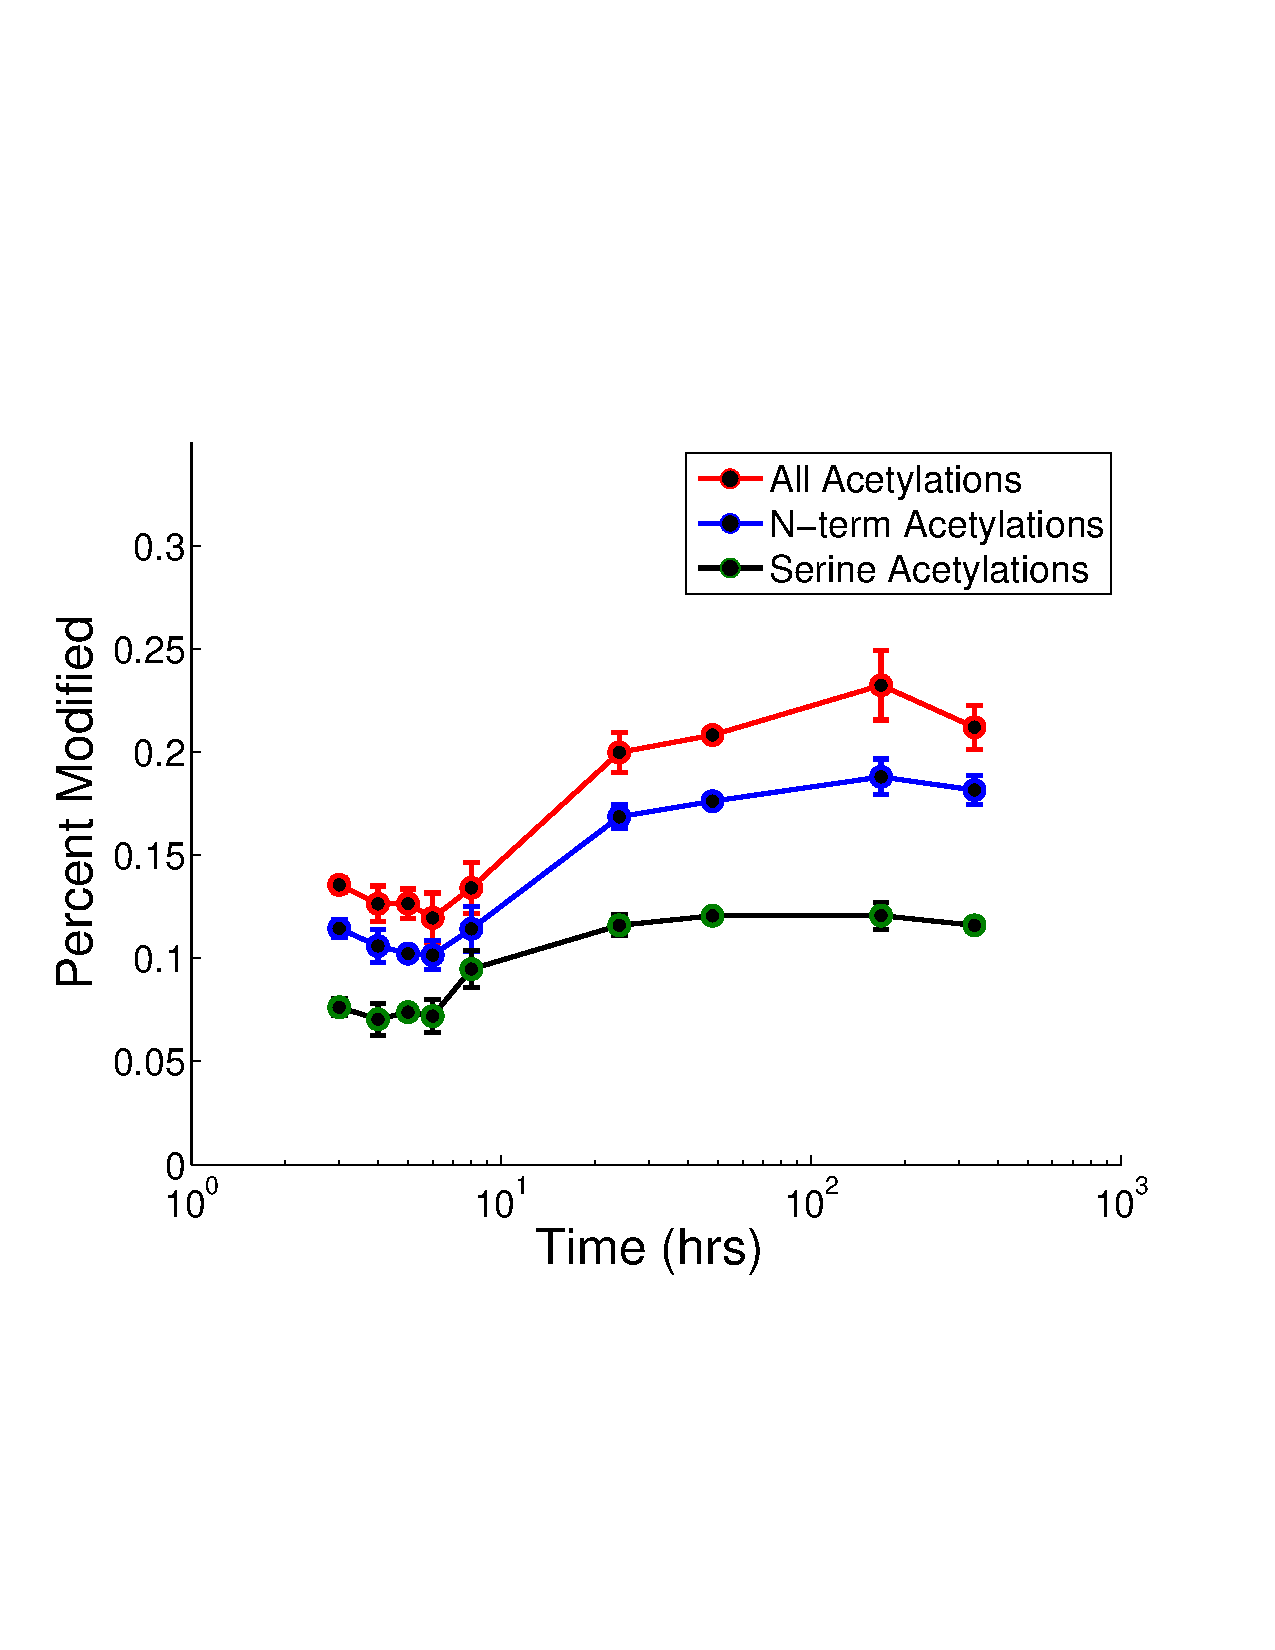
\includegraphics[width=5in]{Figures/Acetylation_AAs.pdf}}
\caption{\label{fig:Acet}\textbf{Protein n-term acetylations are dominant.} Total number of acetylations as well as the n-term/serine acetylations seem to go up over 2 weeks. \emph{E. coli} grown on glucose generally tend to accumulate acetate, perhaps this resulted in increase in acetylations..}
\end{figure}

\clearpage
\begin{figure}[p]
\centerline{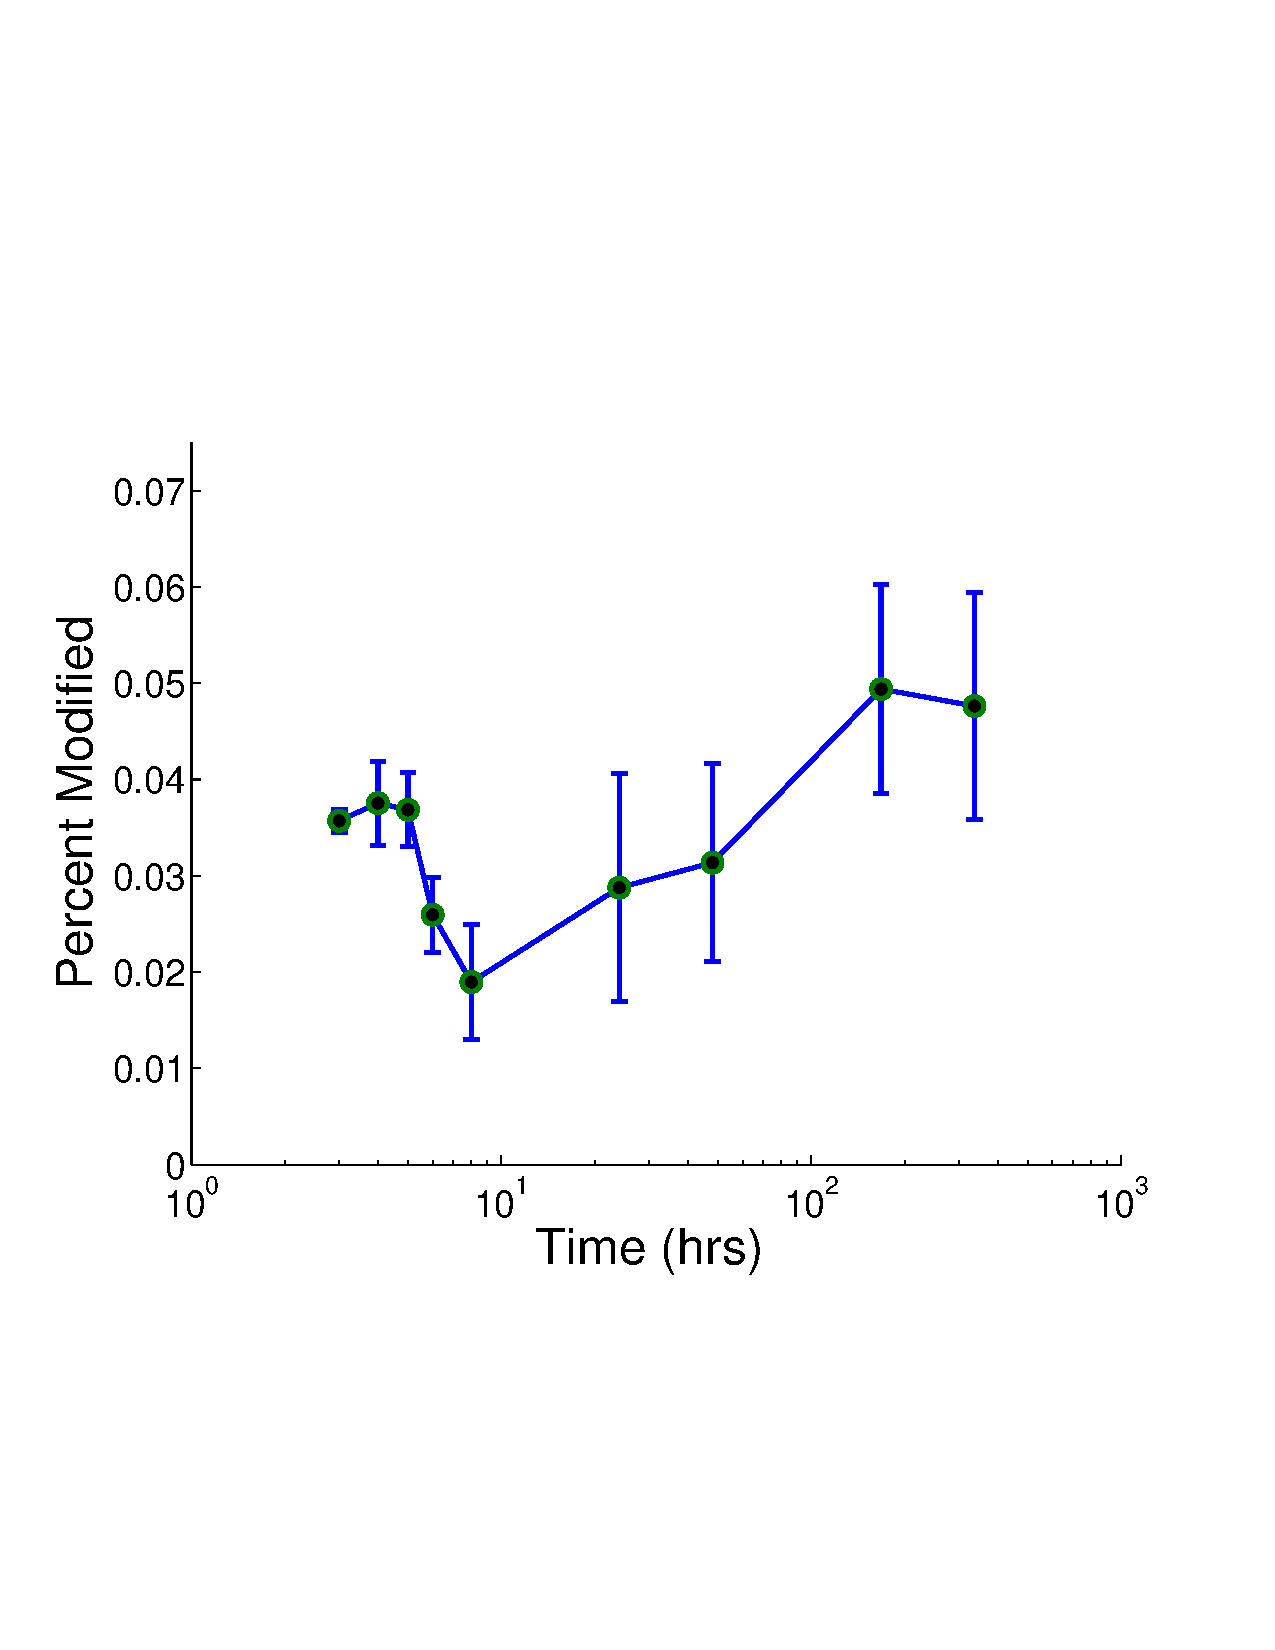
\includegraphics[width=5in]{Figures/Phosphorylations.pdf}}
\caption{\label{fig:Phos}\textbf{Phosphorylations are rare.} Phosphorylations seem to be low and tend to increase during last week of growth. 2 frequently phosphorylated proteins in MODa search output are phosphoglucomutase and elongation factor Tu.}
\end{figure}


\clearpage
\begin{figure}[p]
\centerline{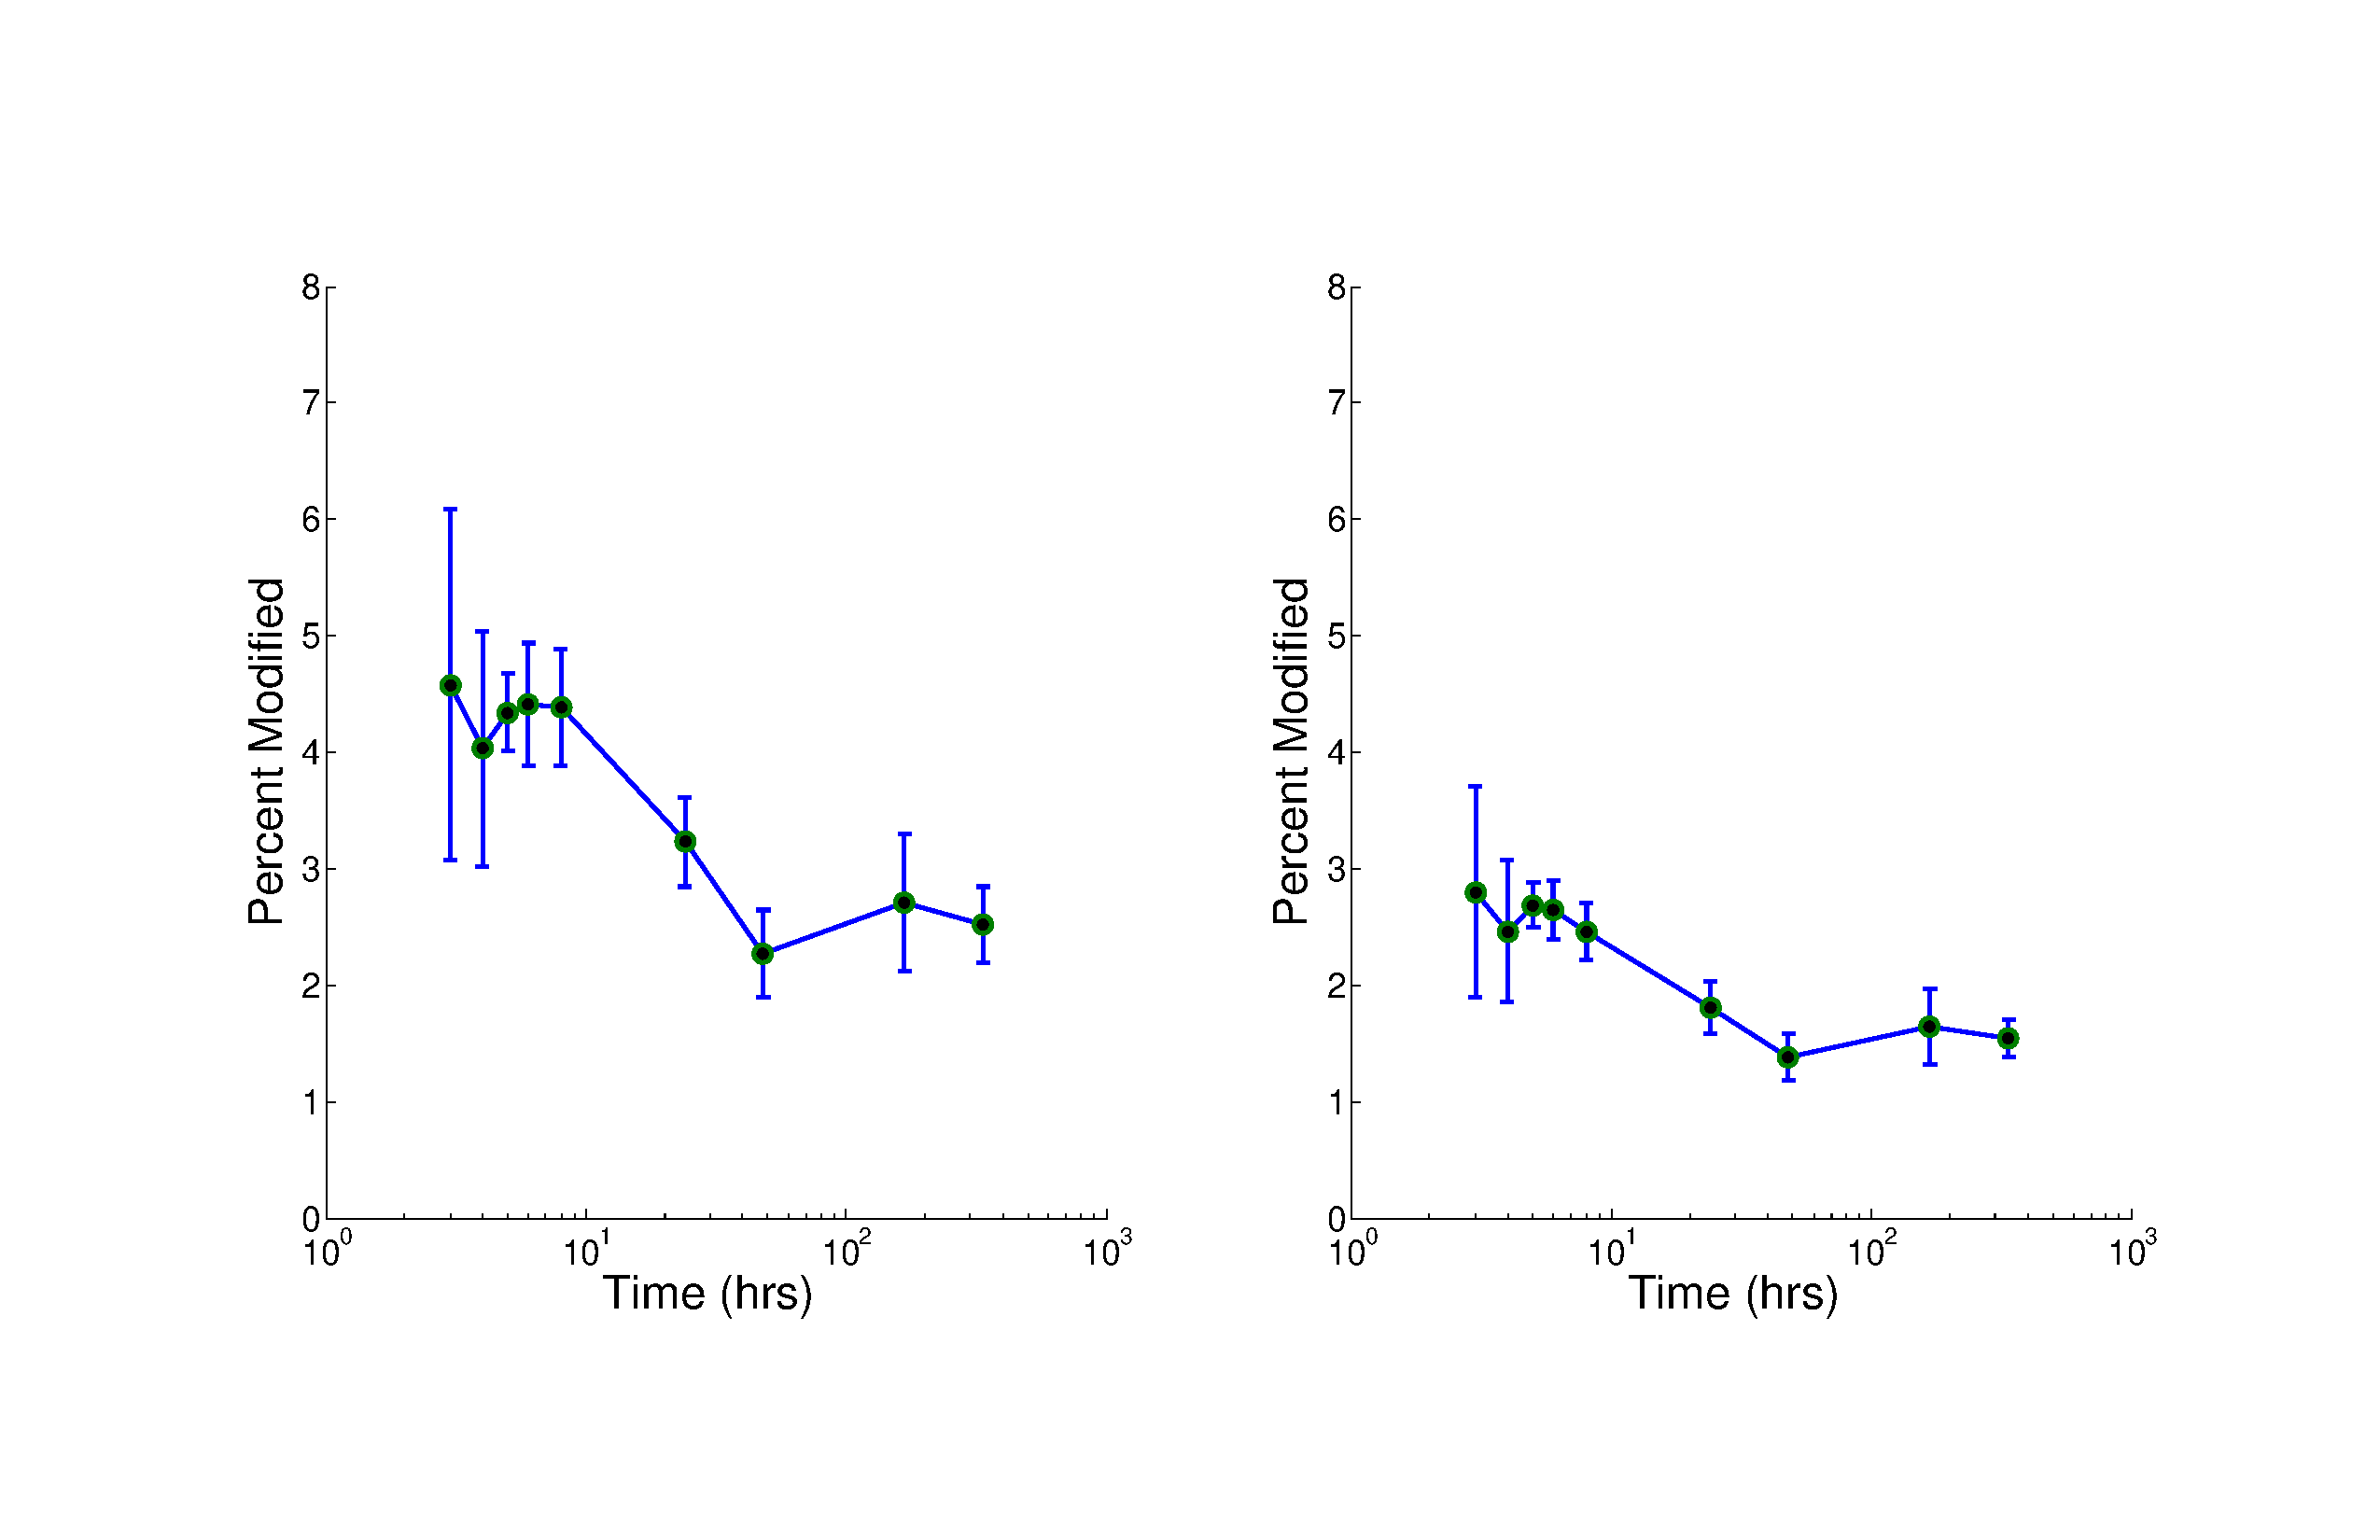
\includegraphics[width=8in]{Figures/Oxidations.pdf}}
\caption{\label{fig:Oxid}\textbf{Oxidations go down over 2 weeks.} (A) Total number of oxidations seem to go down from exponential to stationary phases. (B) The same trend follows for methionine oxidations too.}
\end{figure}

\clearpage
\begin{figure}[p]
\centerline{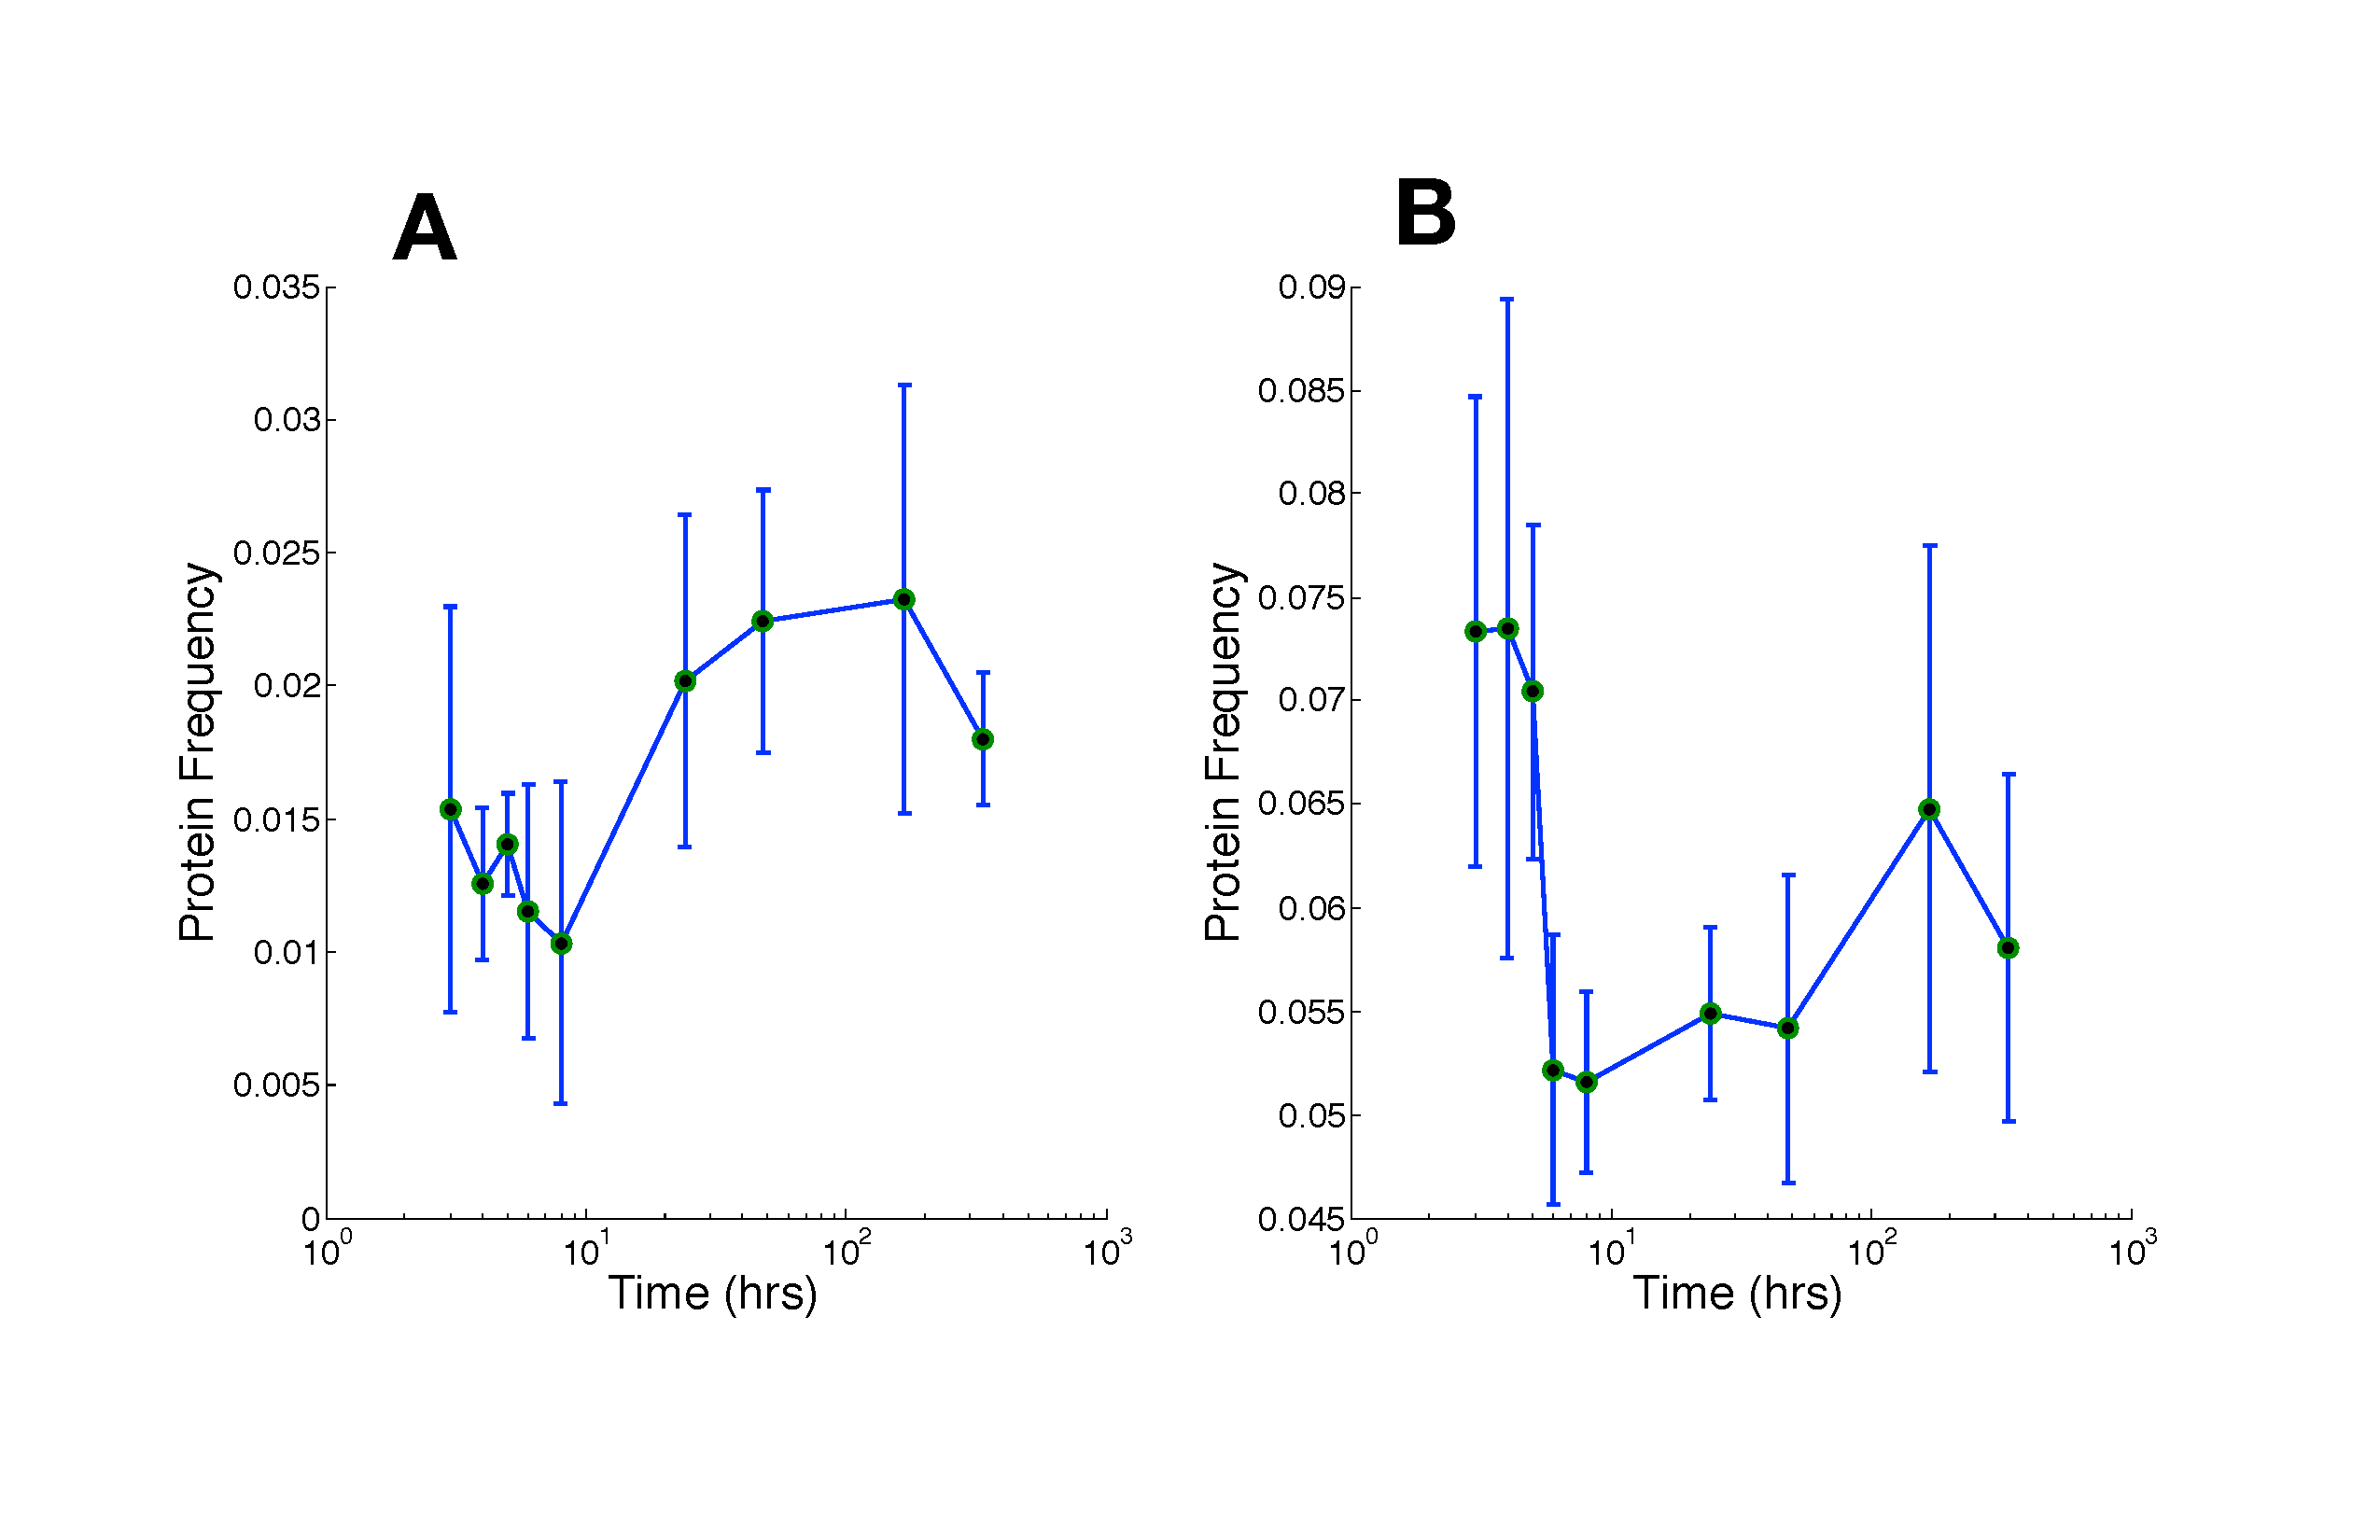
\includegraphics[width=8in]{Figures/Ecoli_MsrAB_MODa.pdf}}
\caption{\label{fig:MsrAB}\textbf{Relative mRNA and protein abundances of methionine sulfoxide reductases MsrA and MsrB.} (A) and (C) mRNA abundances of MsrA and MsrB. The increase of mRNA abundance in stationary phase is not prominent. (B) Protein abundances from 2 different programs seem to agree that MsrA and MsrB are probably fixing methionine sulfoxide to methionine. One of the sites oxidized on MsrA is FQAA[M+16]LAADDDR.}
\end{figure}

\bigskip
\section*{Supplementary Figures}
\clearpage
\centerline{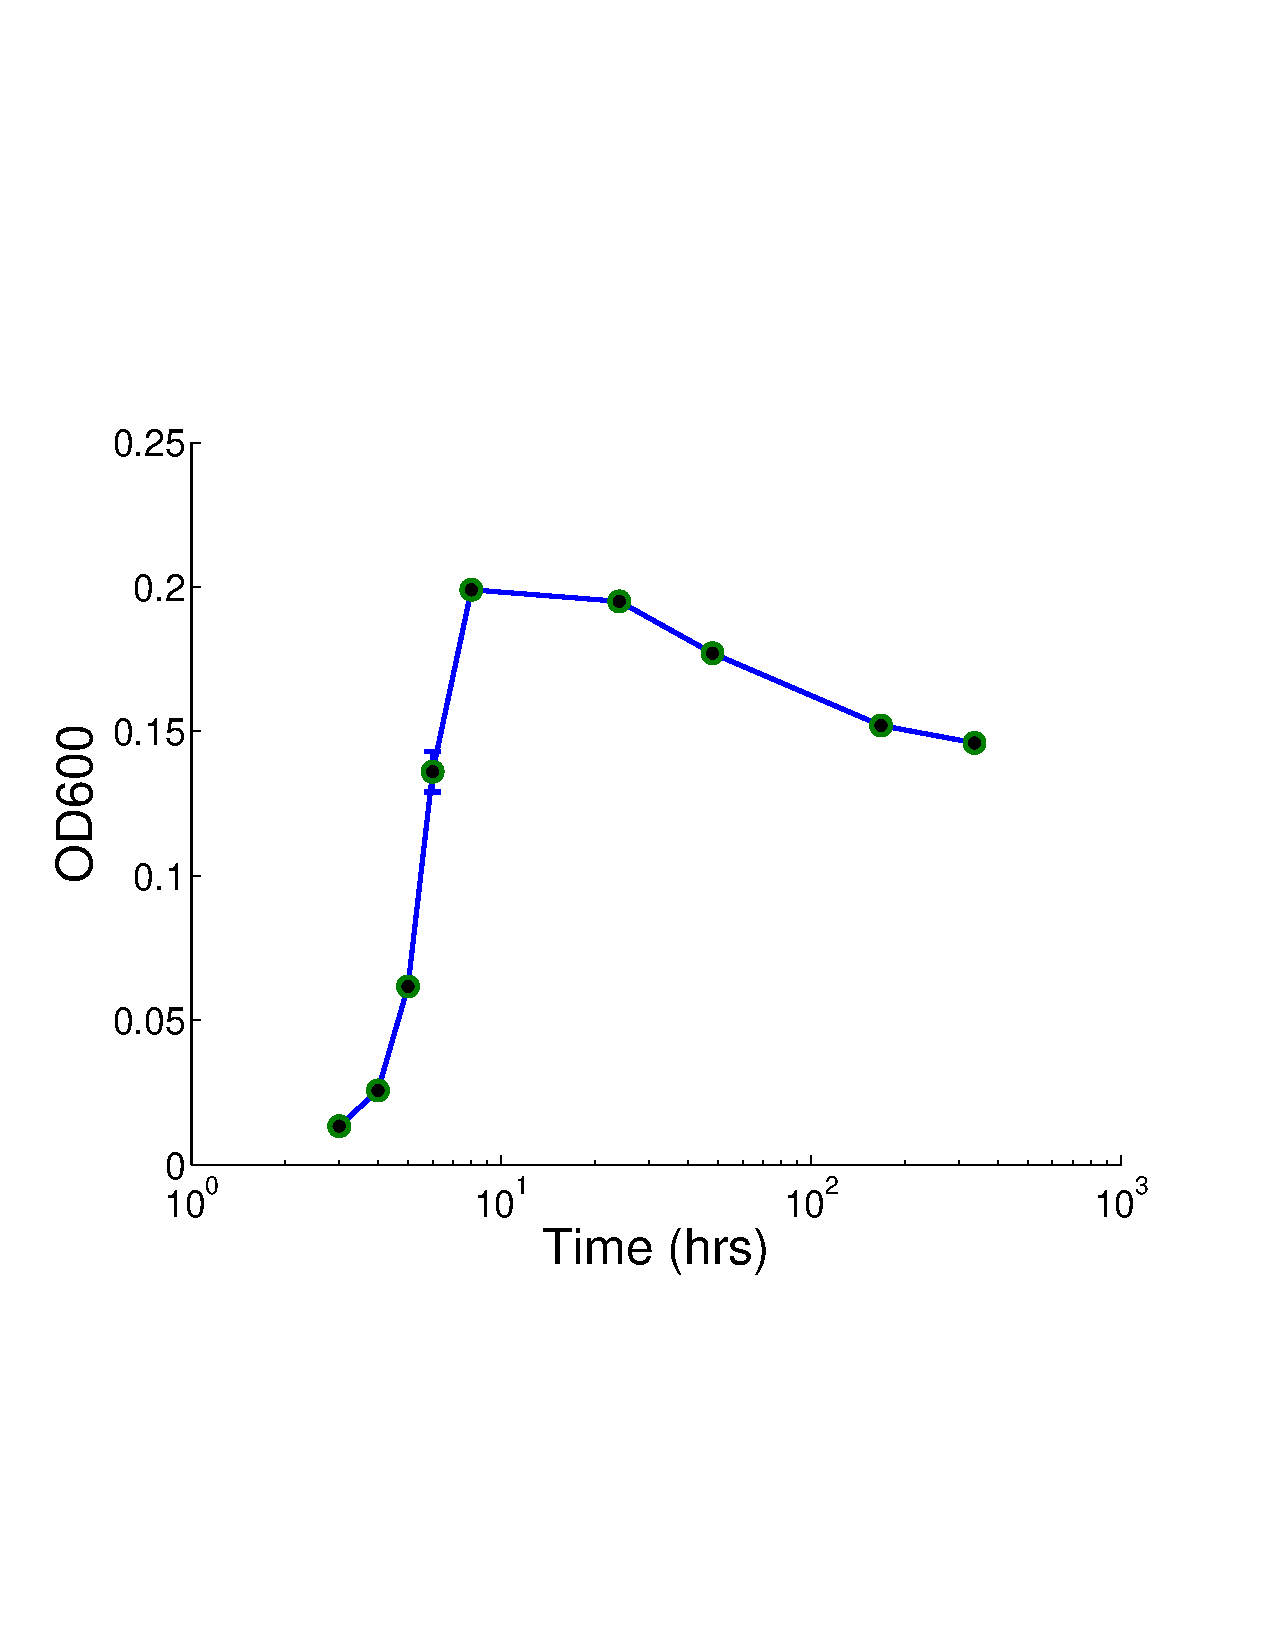
\includegraphics[width=5in]{Figures/GrowthCurve.pdf}}
\customlabel{fig:GrowthCurveFig}{S1}
\textbf{Figure S1: OD600 curve .}  Growth curve (OD600) of REL606 under glucose starvation conditions.

\clearpage
\centerline{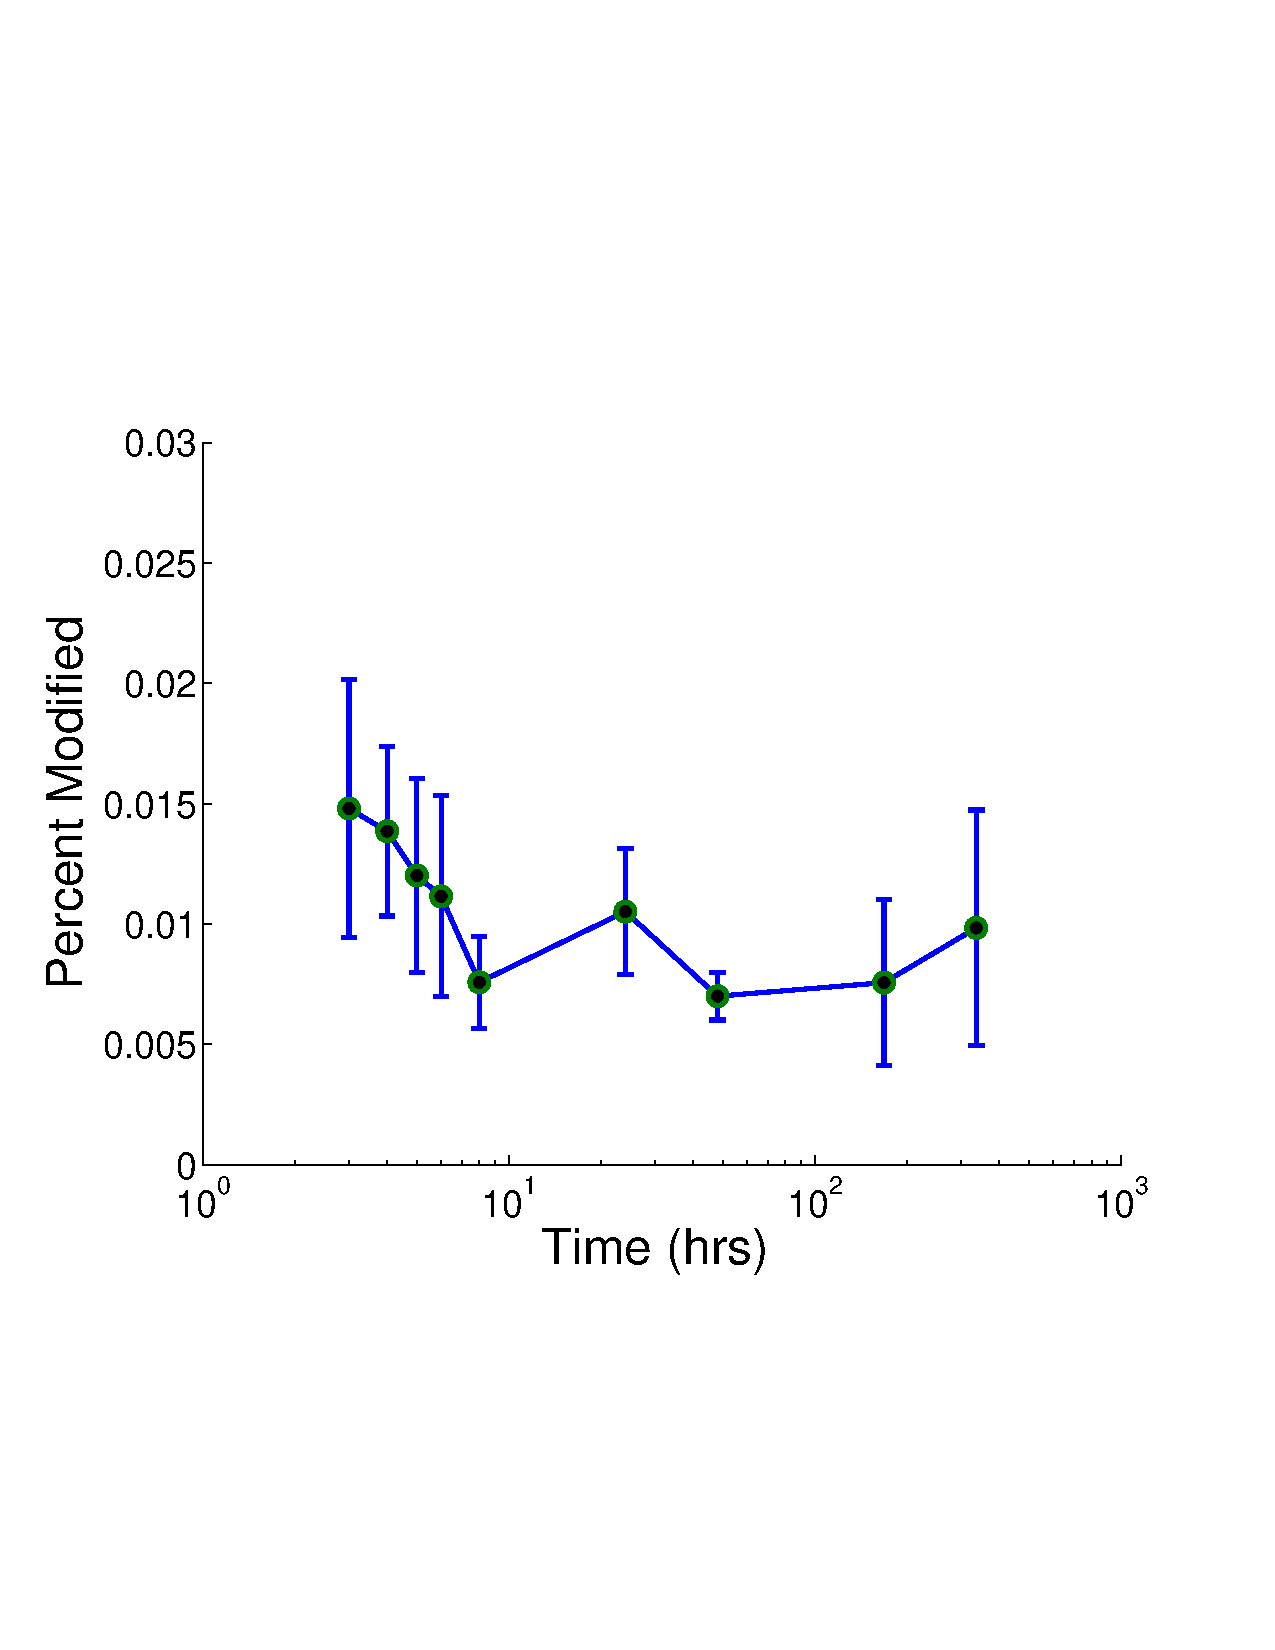
\includegraphics[width=5in]{Figures/Nitrosylations.pdf}}
\customlabel{fig:NitrosylationFig}{S2}
\textbf{Figure S2: E. coli Nitrosylations.} Nitrosylations seem to go down.

\clearpage
\centerline{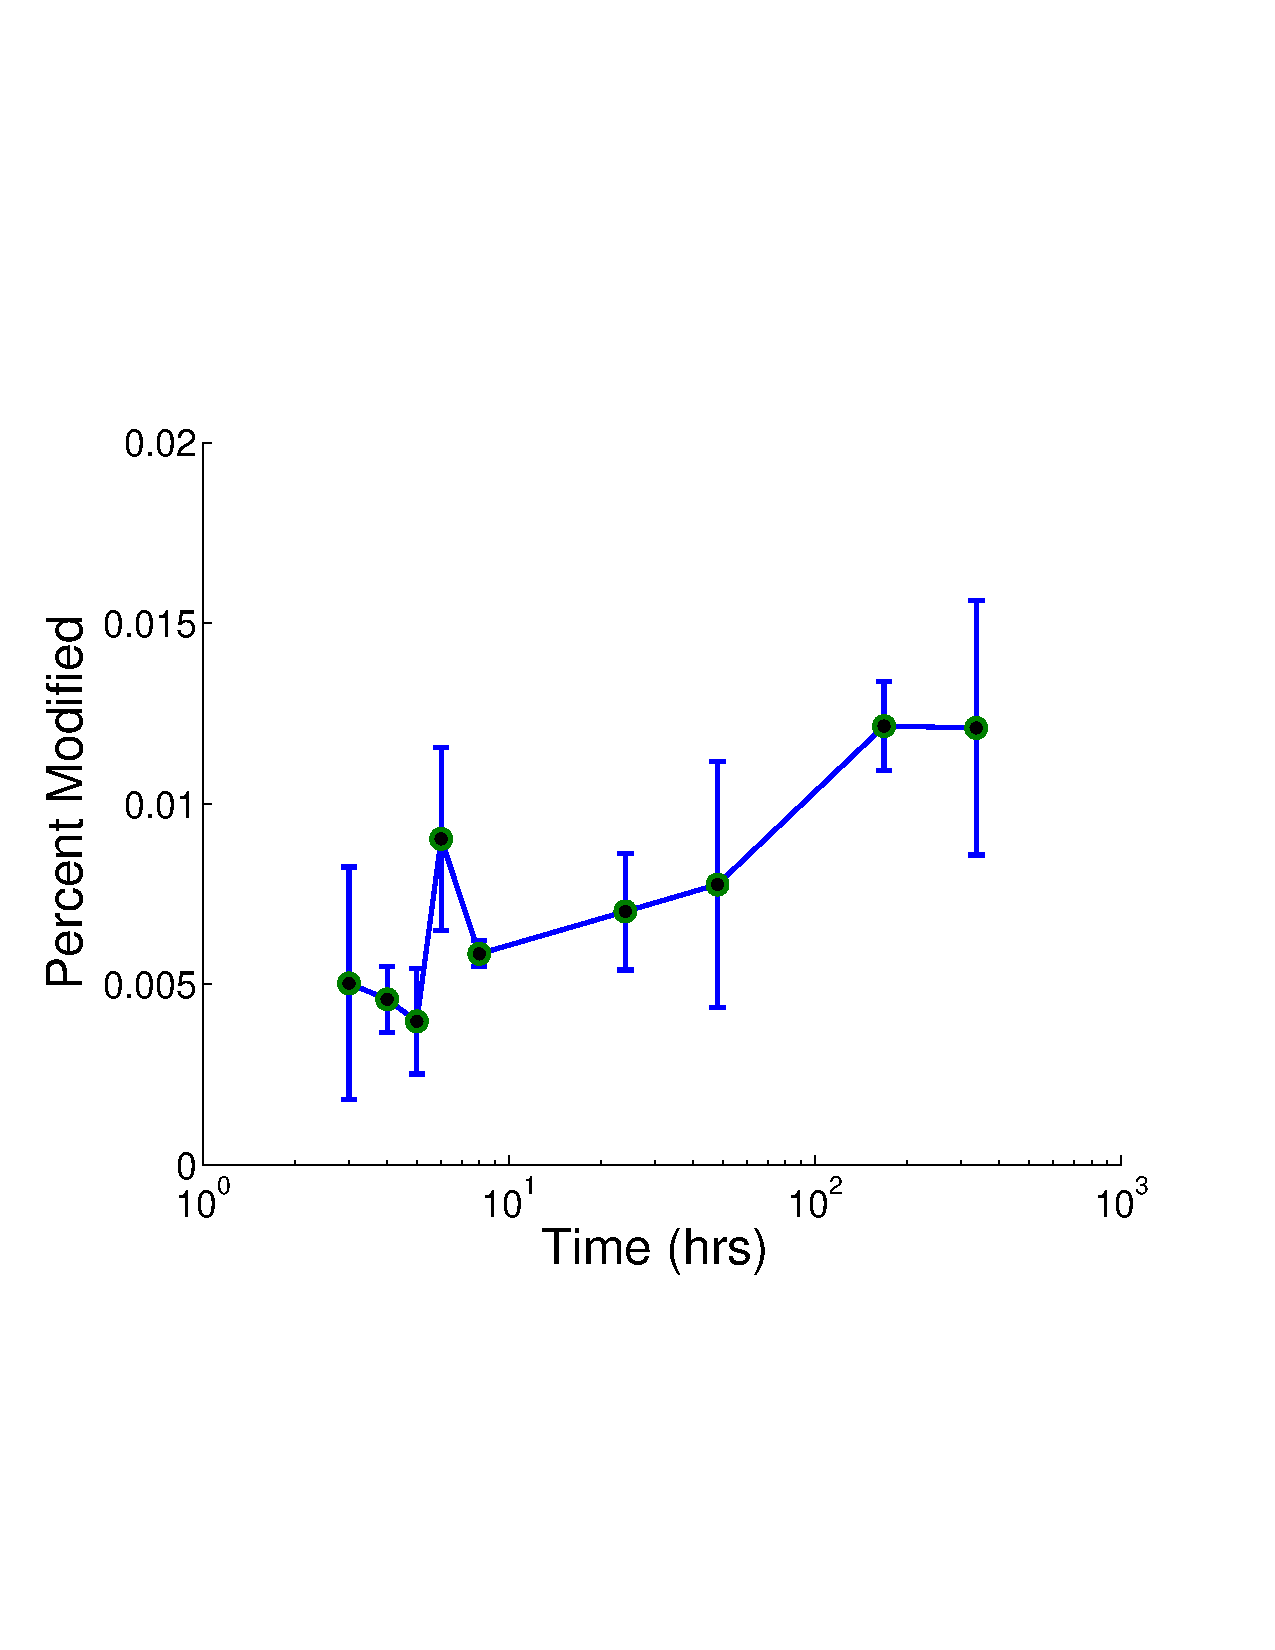
\includegraphics[width=5in]{Figures/Carboxylations.pdf}}
\customlabel{fig:CarboxylationFig}{S3}
\textbf{Figure S3: E. coli Carboxylations .} Carboxylations seem to go up.

\clearpage
\centerline{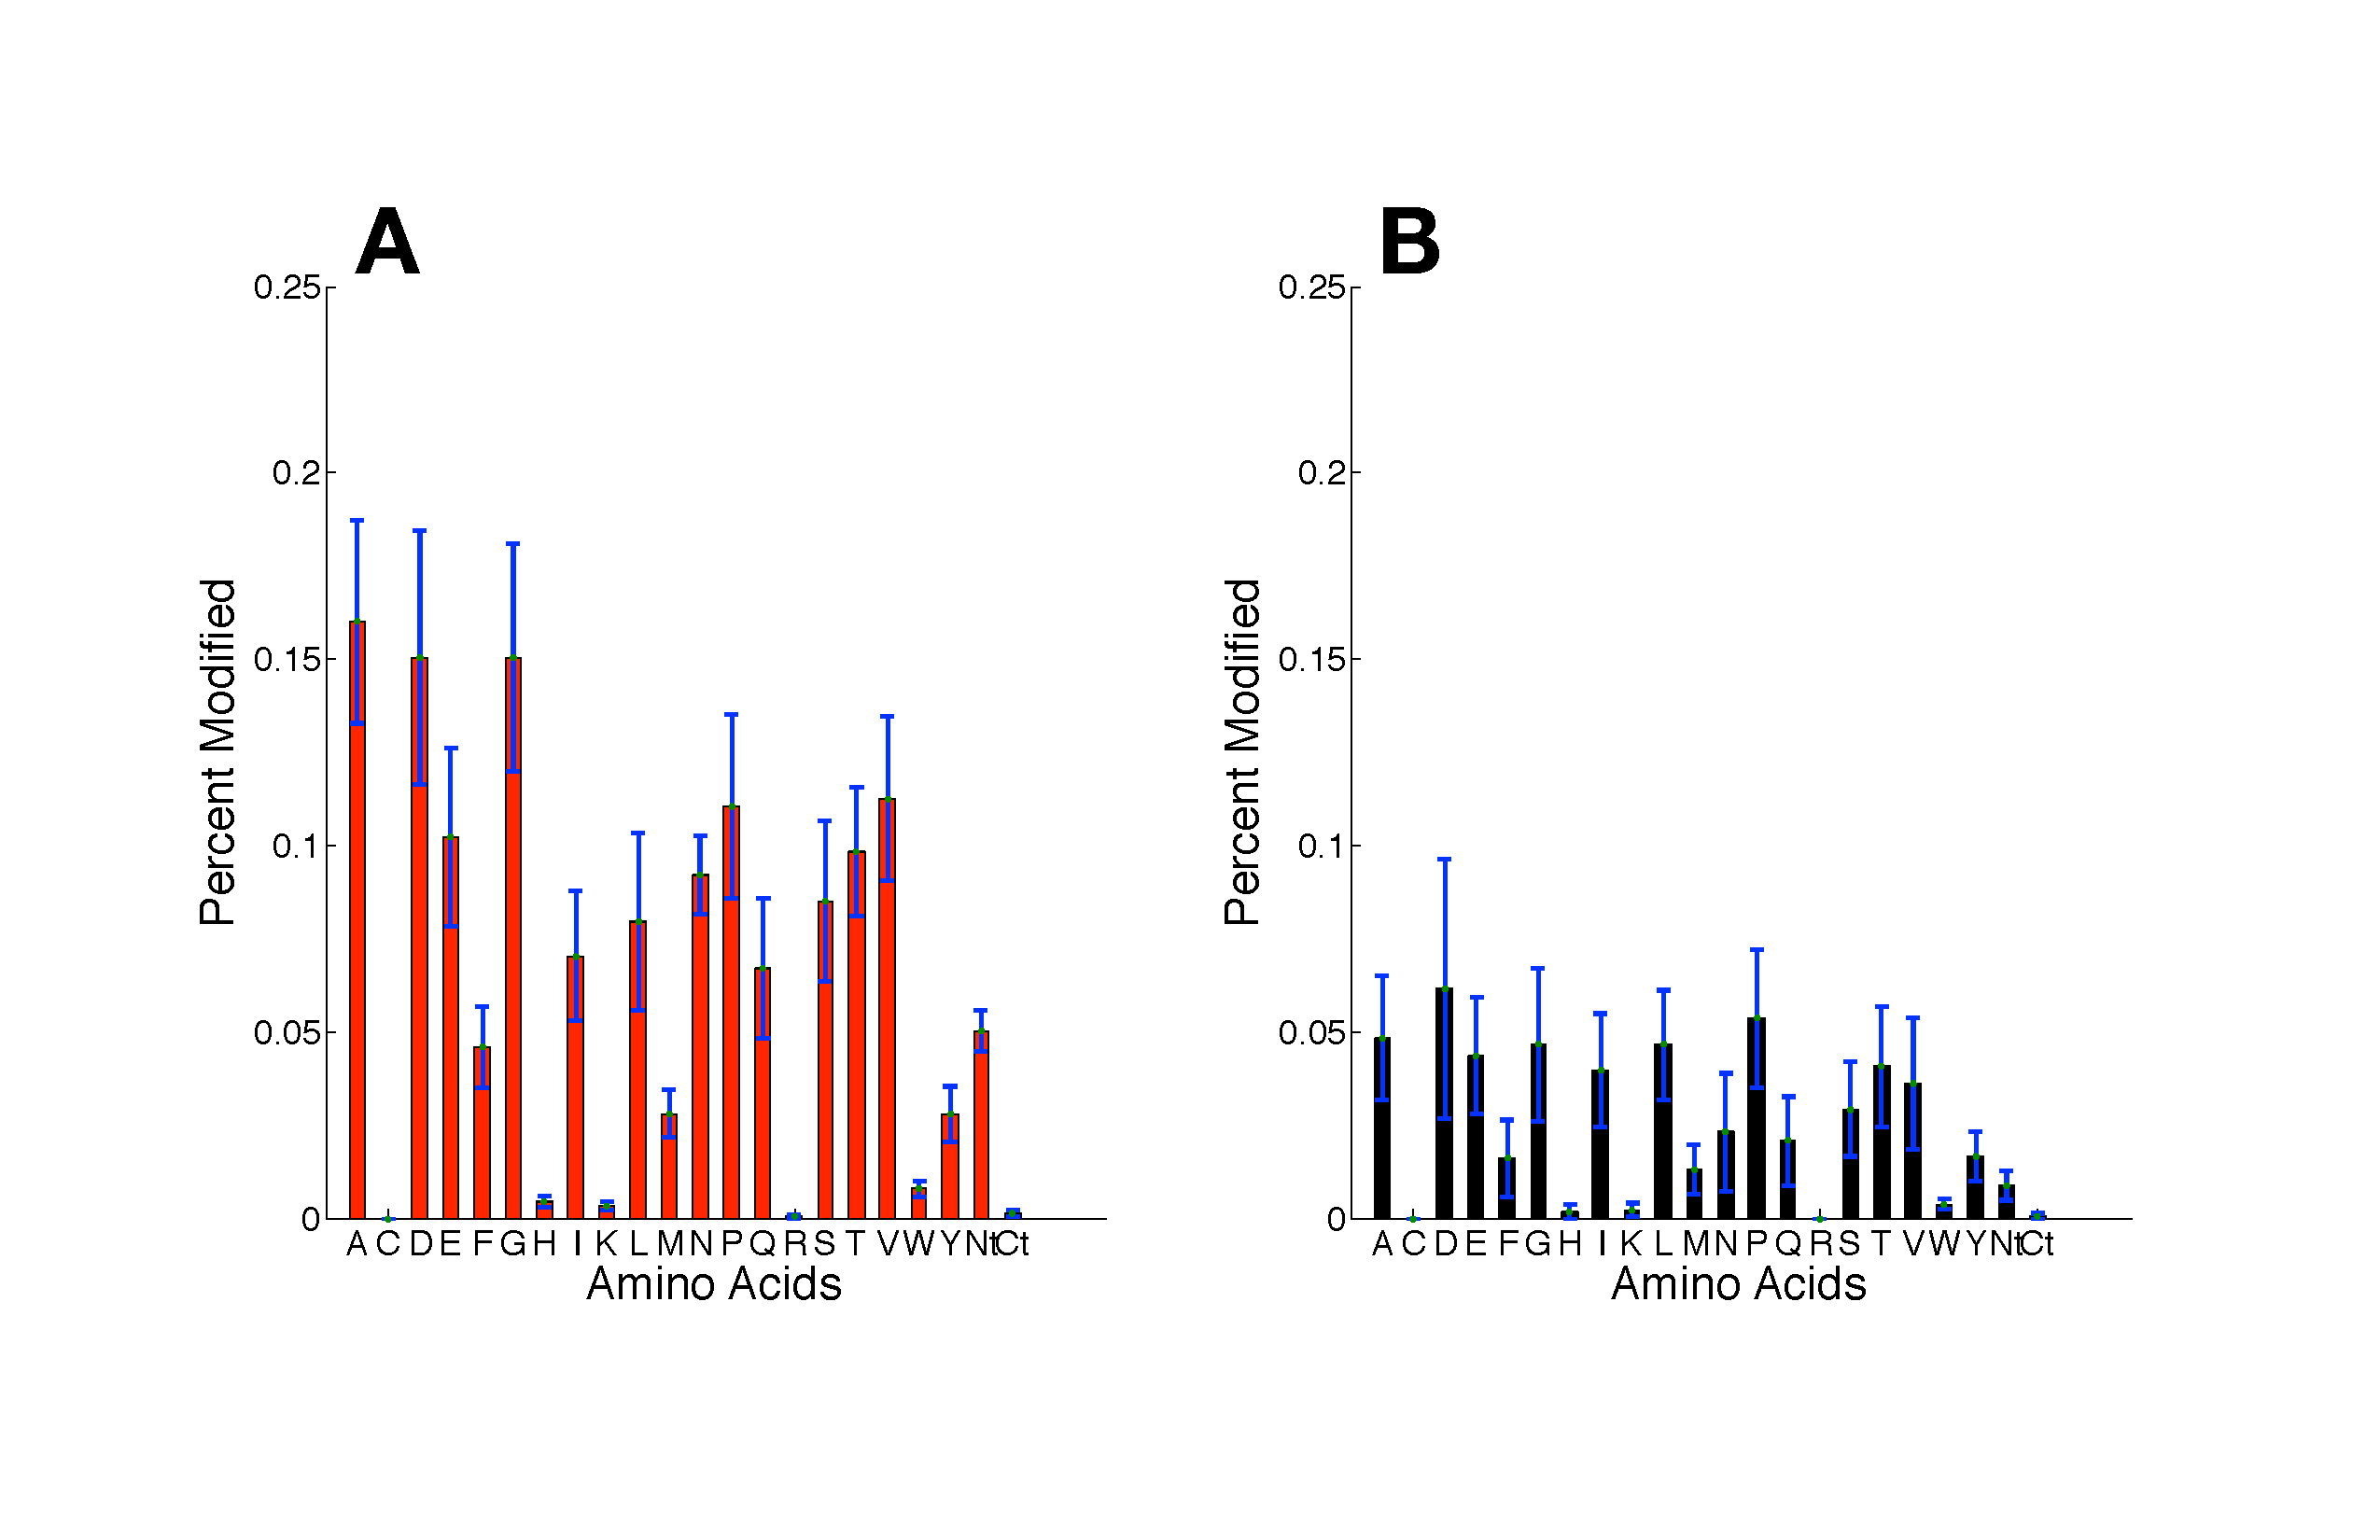
\includegraphics[width=8in]{Figures/NaKAdducts.pdf}}
\customlabel{fig:CarboxylationFig}{S4}
\textbf{Figure S4: Na and K adducts.} Na and K adducts seem to happen on all amino acids except those that are basic and carry some charge, as expected.

\clearpage
\centerline{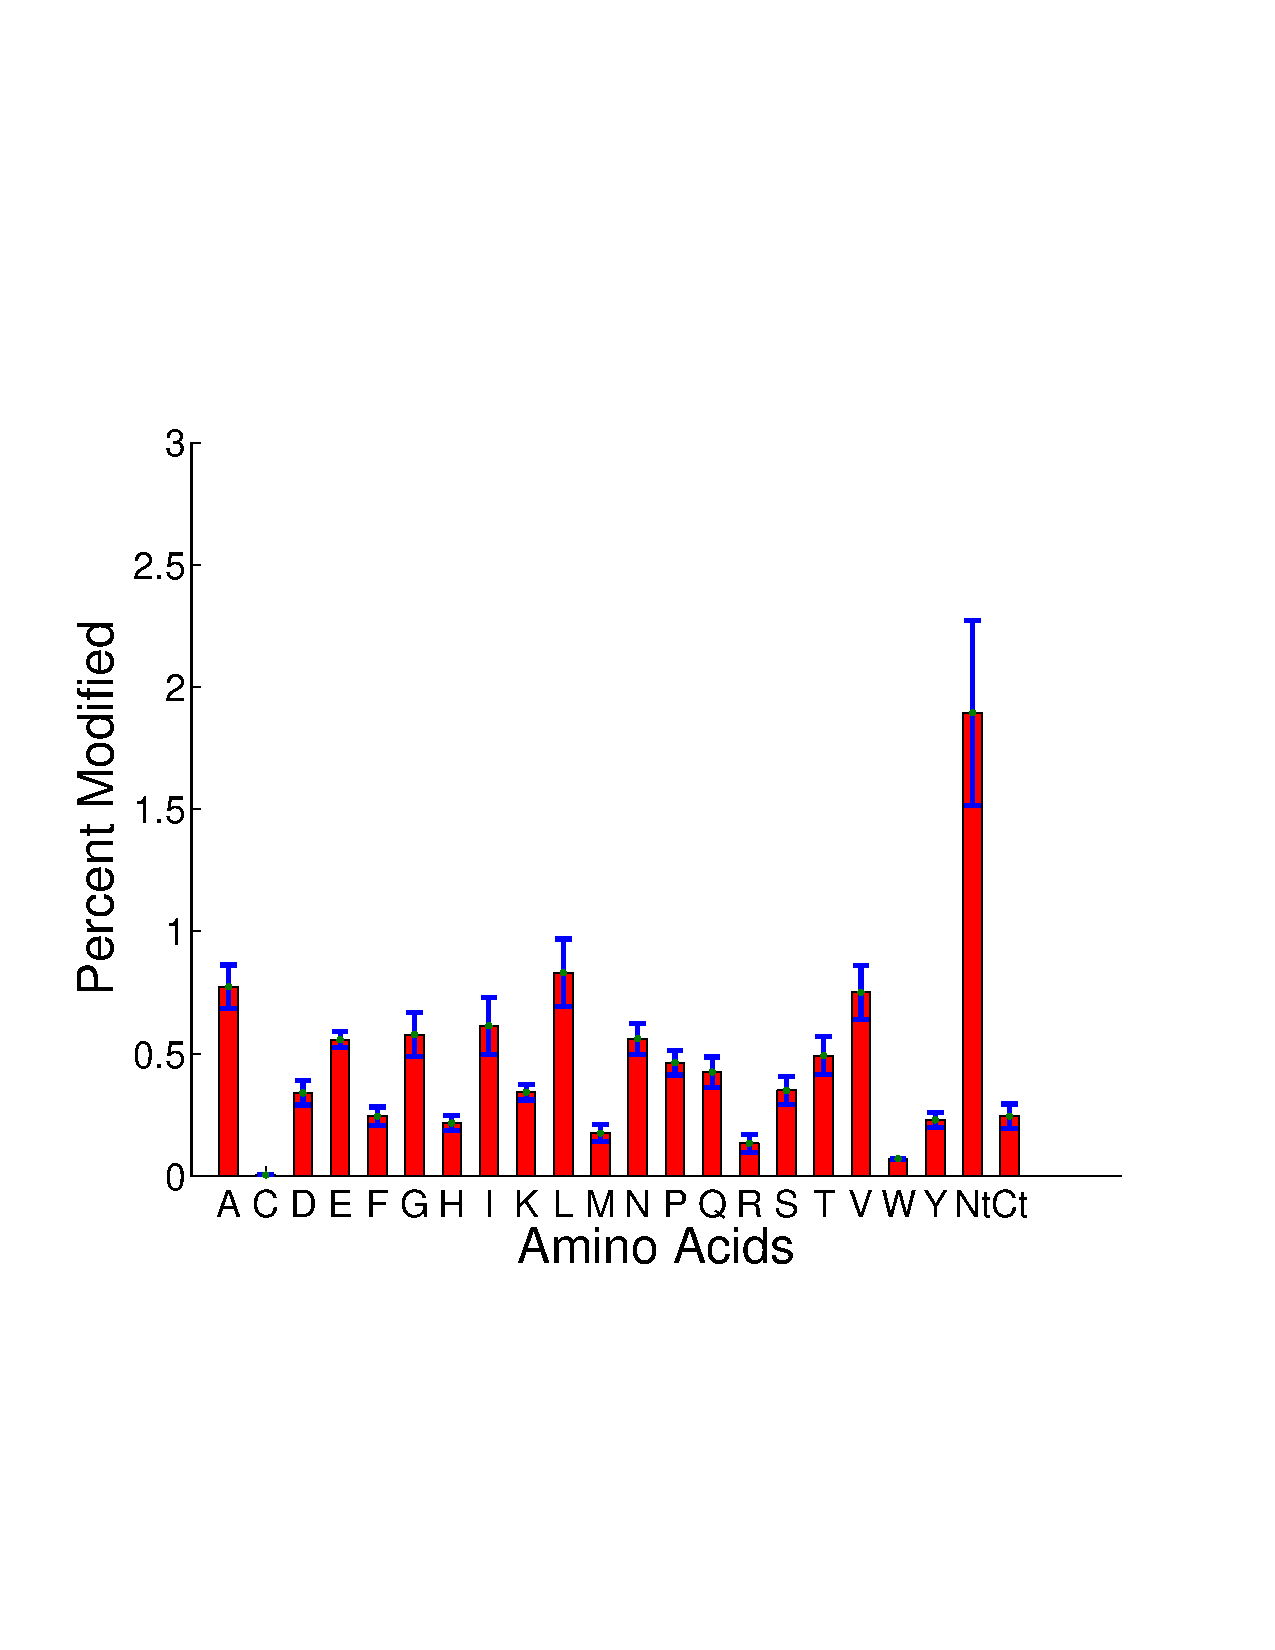
\includegraphics[width=5in]{Figures/1DaProfile.pdf}}
\customlabel{fig:1DaProfileFig}{S5}
\textbf{Figure S5: +1Da shift occurs randomly.} We cannot infer that this is deamidation as it occurs randomly on all amino acids, inferring it is mostly 13C peak picking as previously shown in many studies. 

\clearpage
\centerline{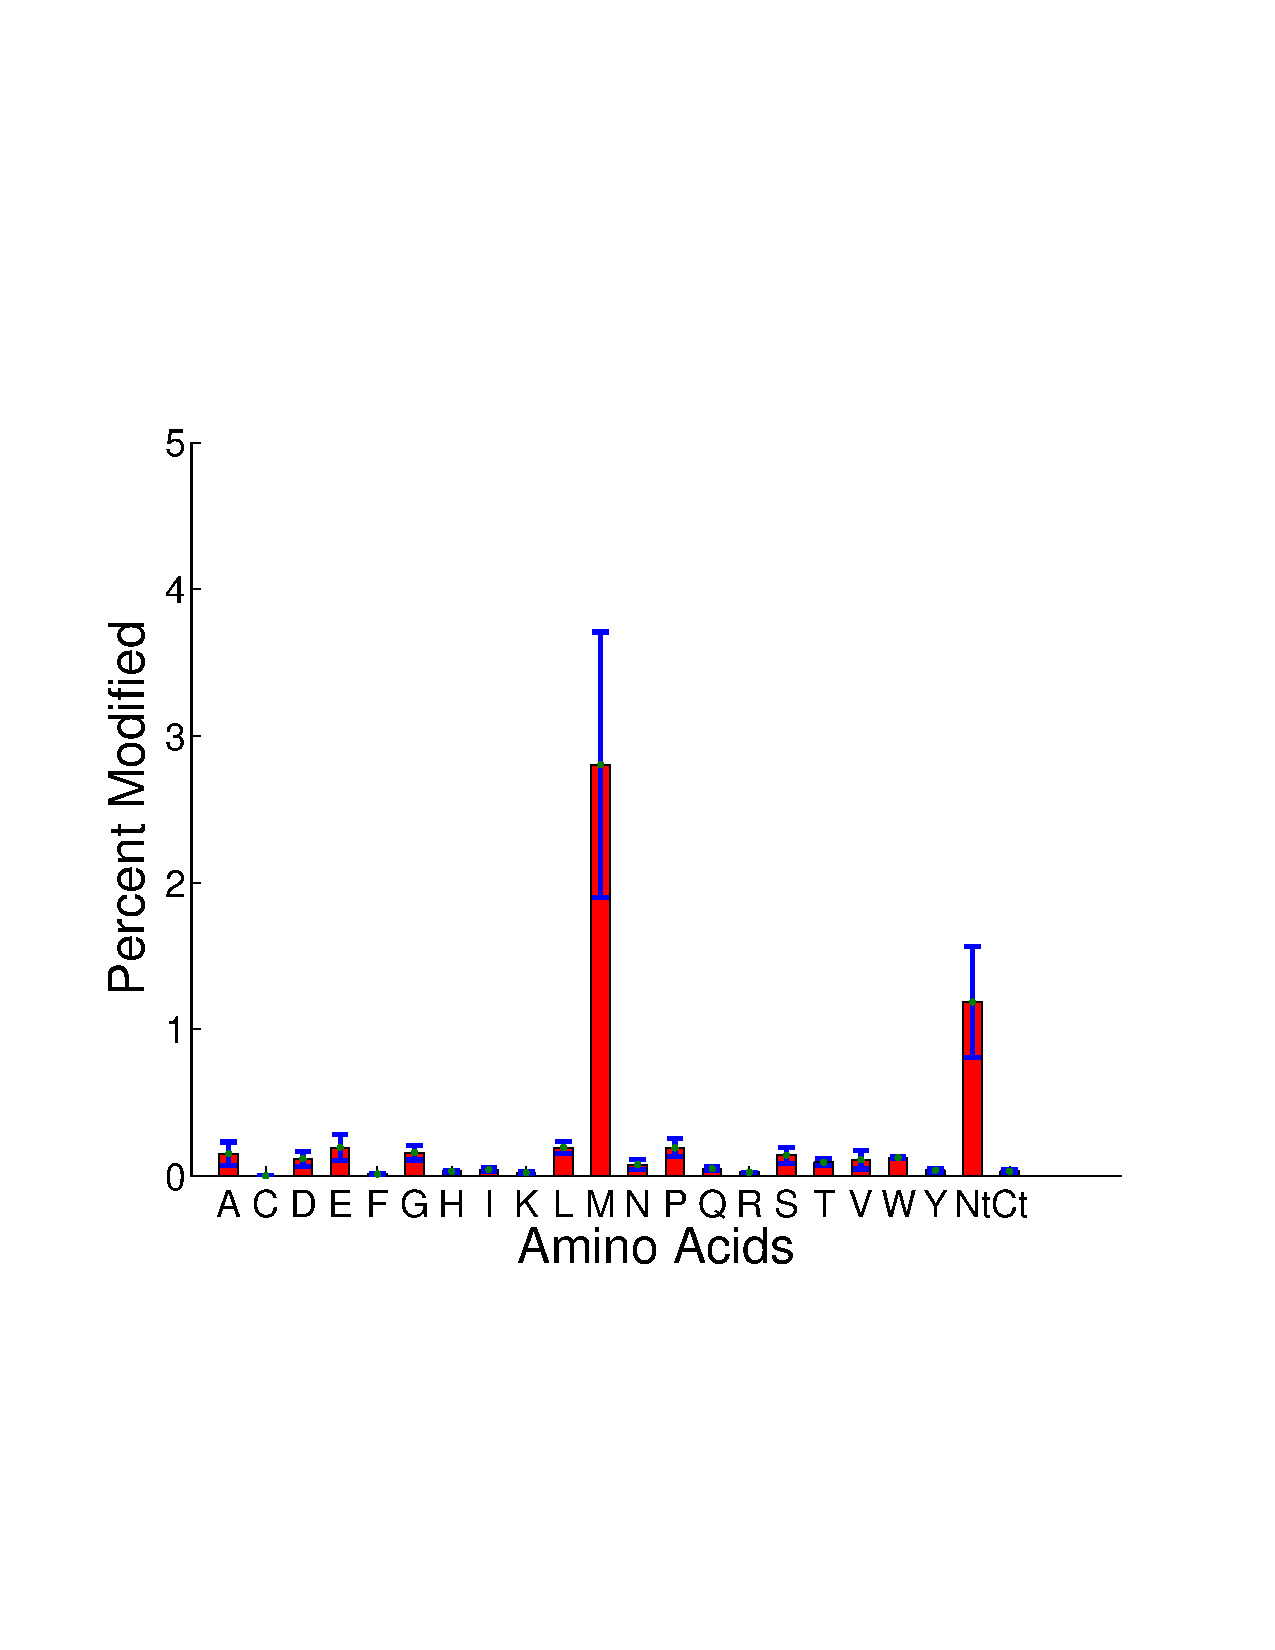
\includegraphics[width=5in]{Figures/OxidationProfile.pdf}}
\customlabel{fig:OxidationProfileFig}{S6}
\textbf{Figure S6: Oxidation is dominant on methionine.} Even though many amino acids could be oxidized, in this data set, oxidation seems to occur primarily on methionine, as expected. 

\clearpage
\centerline{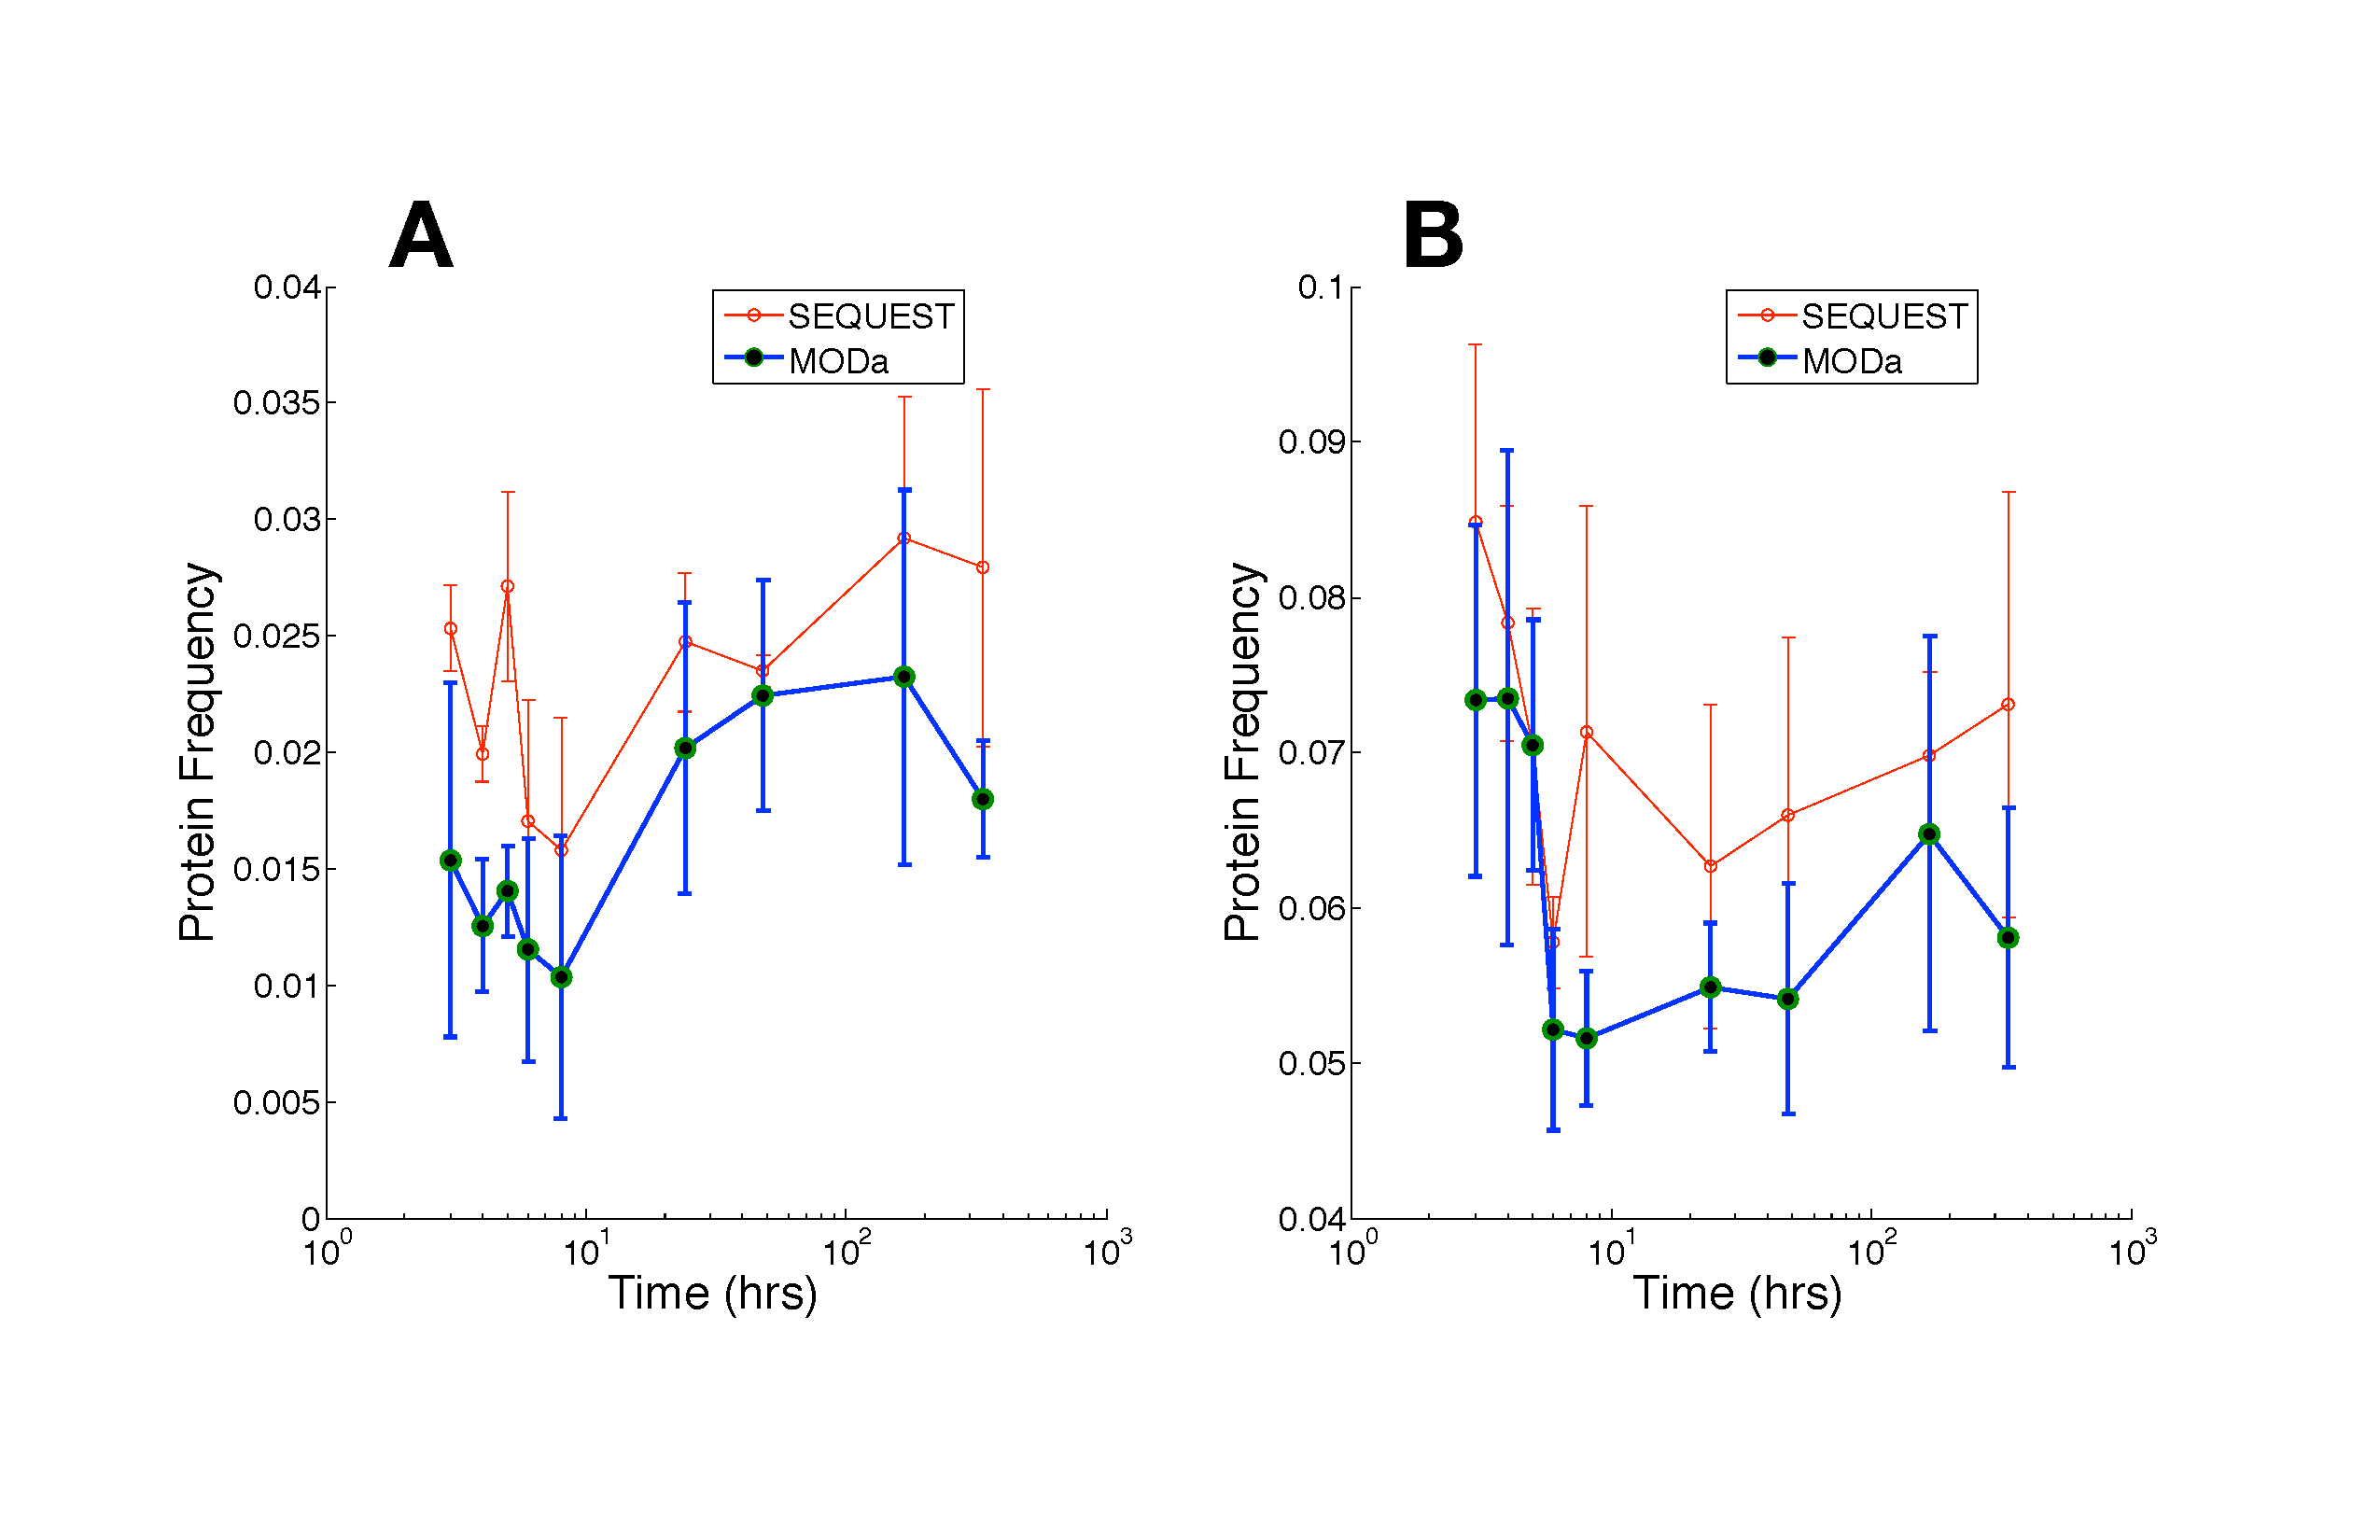
\includegraphics[width=8in]{Figures/Ecoli_MsrAB_MODa_Sequest.pdf}}
\customlabel{fig:OxidationProfileFig}{S7}
\textbf{Figure S7: Oxidation is dominant on methionine.} Even though many amino acids could be oxidized, in this data set, oxidation seems to occur primarily on methionine, as expected.

\clearpage
\centerline{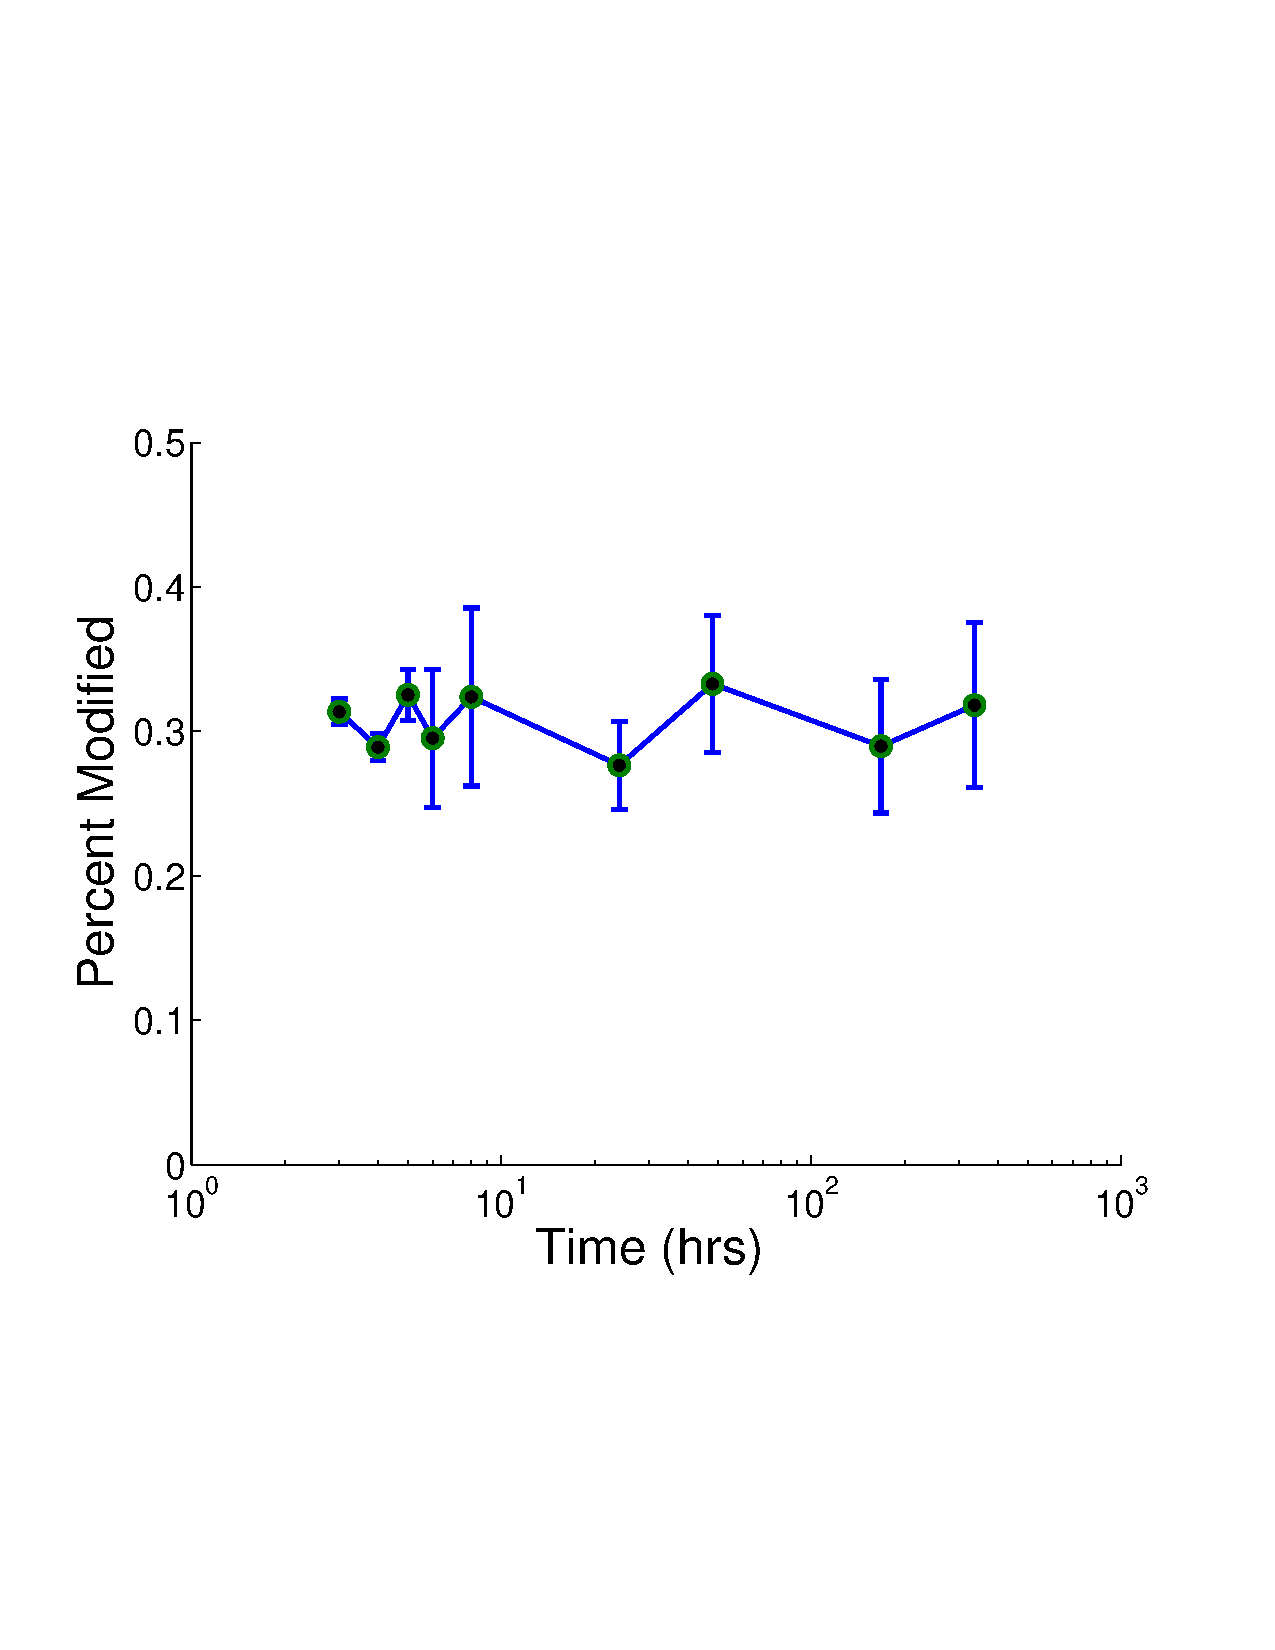
\includegraphics[width=5in]{Figures/PyroGlutamate.pdf}}
\customlabel{fig:1DaprofileFig}{S8}
\textbf{Figure S8: Glutamine to pyroglutamate conversion.} Glutamine to pyroglutamate happens to stabilize the protein. This conversion seems to be consistent across both the exponential and stationary phases. 

%\section*{Supplementary Tables}
%\customlabel{tab:predictive_carbon_sources}{S1}
%\textbf{Table S1: .} These .
%\bigskip

%\noindent File: \texttt{SupportingInfo/CarbonSources.xlsx}\\
%Available in github repository \texttt{https://github.com/clauswilke/Ecoli\_FBA\_input\_prediction}

%\bigskip
%\customlabel{tab:predictive_nitrogen_sources}{S2}
%\noindent \textbf{Table S2: .} These .
%\bigskip

%\noindent File: \texttt{SupportingInfo/NitrogenSources.xlsx}\\
%Available in github repository \texttt{https://github.com/clauswilke/Ecoli\_FBA\_input\_prediction}

\end{document}
